\chapter{Use cases for capacitive proximity sensors}
\label{ch:usecases}
After having defined the potential application domains for capacitive proximity sensors, in the following section I would like to evaluate the actual use cases by presenting associated challenges, presenting data processing methods on how to tackle these, and present a number of prototypes that have been created implementing these methods. This allows to gather the information required to discuss the application of capacitive proximity sensors in smart environments and validate their use in Chapter \ref{ch:eval}. In addition to the application specific challenges there are also numerous implementation challenges that are detailed in the descriptions of the associated prototypes.
\section{Use cases and associated challenges}
Looking at the previously defined application domains for capacitive proximity sensing, we can get more specific and derive actual use cases that belong in the different domains. While it would be possible to associate the different systems presented in the related works, this approach would not allow to capture actual challenges in the application process, apart from the discussion within the specific work. Thus, I am focusing on the implemented prototype systems that will be presented in the subsequent sections. Table \ref{tab:usecase_list} shows the different application domains, how capacitive proximity sensors can be applied, and the use cases that were derived from it. In this section I will discuss how this table was derived and create a list of challenges that become apparent when designing the specific systems. Based on these challenges it is possible to identify a number of improved and new methods in the processing of capacitive proximity sensor datam that are required to design the presented applications. These specific contributions to the processing methods will be detailed in the following section.

% Table generated by Excel2LaTeX from sheet 'Tabelle1'
\begin{table}[htbp]
  \centering
  \caption{Application domains and derived implemented use cases for capacitive proximity sensing}
    \begin{tabularx}{\linewidth}{p{3.5cm}XX}
    \toprule
    Application Domain & Applying capacitive proximity sensors & Implemented use cases \\
    \midrule
    Indoor Localization & Sensing system hidden in environment & Capacitive sensing below floor cover \\
    Smart Appliances & System detecting presence and other parameters of human bodies in range & Posture recognizing office chair, occupation sensing bed, arm detecting armrest \\
    Physiological Sensing & Determine physiological parameters associated to movement & Breathing rate detection via chest movement, long-term movement analysis \\
    Gesture Interaction & Hand interaction in near range & Finger gestures, single hand 3D gestures, combined multi-hand and touch tracker \\
    \bottomrule
    \end{tabularx}%
  \label{tab:usecase_list}%
\end{table}%



Indoor localization has been presented as one of the application examples for smart environments in the related works section. The main advantage of capacitive systems is their unobtrusive application in the environment as presented in TileTrack \cite{Valtonen2009a} and SensFloor \cite{lauterbach2009}. Capacitive indoor localization systems can be hidden below any non-conductive material and enable tracking of users on a distance. Particularly interesting is the ability to place the sensing equipment below the floor cover as an additional layer, e.g. when installing a new carpet or wood parquet. SensFloor as commercially available solution is designed to be placed as an additional layer and integrates sensors and communication systems therein. While this enables precise sensing close to the walking persons, it is costly and can lead to maintenance issues once the sensors integrated in the layer fail. Instead, it is also a viable option to separate sensor hardware and electrodes, e.g. by placing the sensors on the borders of the indoor area and use a specific electrode layout below the floor. The electrodes can be made of any conductive material and can be insulated using non-conductive isolation to prevent corrosion and physical damage. The system components that are most prone for failure are the connections between electrode and sensor and the sensor hardware and its communication channels. Those can e.g. be placed within the border covers.

The main challenge of this solution is to balance the number of sensors and the intended resolution. Using a limited set of sensors placed on the border it should nonetheless be possible to determine the positions of one or more persons on the area above. Preferably additional information should be gathered, e.g. if a person is standing, sitting or lying. In addition to the cost factor, a larger number of sensors also causes several other issues. One example is cross-talk between the different electrodes that has to be avoided using a variety of multiplexing methods. The achievable resolution of the single electrodes is depending on several factors, including the measurement time, the applied voltage, distance between electrodes and floor surface, or the geometric layout of the electrodes. Thus, it is important to find an electrode layout and processing methods that achieve this balance.

Smart appliances as presented in the related works comprise a very diverse group of devices that are in the current environment. There is a huge variety of sensor categories and processing that can be applied to any given task. Looking at capacitive proximity sensors, the major advantage is the invisible application that allows to create smart appliances that are indistinguishable from non-equipped systems. Using different conductive materials for the electrodes this integration can range from solid antennas hidden within the appliance to conductive threads that can be woven into fabric. The main application for capacitive proximity sensors in smart appliances is the sensing of different parameters of persons interacting with the system. For example the sensors can be used to recognize the posture of a user and use it to adapt certain parameters of the appliance or the environment. This type of interaction has also been called implicit interaction, as the user does not directly attempt to manipulate the environment, but instead the activities are interpreted as input according to the given situation \cite{schmidt2001build}. In many instances it is sufficient to get information about the presence of the user. A simplified posture recognition can be used to detect presence or occupation, based on the data acquired by one or more sensors. Finally, it is often also interesting to detect if certain body parts are currently at a given location, e.g. the arm resting on the armrest of a chair, indicating a specific situation that the system can react on.

The challenges in this domain are manifold. Existing posture recognition systems might rely on a different sensor category, supporting hundreds of measurement spread over a larger area. Again, capacitive proximity sensors are distributed sparsely and need methods that enable gaining a similar amount of higher-level information. Here it is necessary to create models of the human body that are suited for the processing of capacitive data. According to the parameters that are supposed to be detected the models can be more or less complex and thus optimize the required processing time. A sensing bed that has to detect if a person is lying would require a simpler model, as opposed to a sensing chair that has to detect a larger variety of different postures. Often the capacitive systems are combined with other systems, or use a custom non-uniform distribution of electrodes in the device that require methods of data fusion and processing of heterogeneous signals to acquire higher level information, e.g. an armrest that combines the detection of an arm and an interactive area that allows gesture interaction.

Physiological sensing allows us to measure signals generated by the different process of the human body. One common application the tracking of training effects by athletes. This may include measuring heart rate or respiration. There are numerous medical applications ranging from long-term blood pressure sensing, to blood glucose level sensing or tracking the quality of sleep throughout the night. Additionally, there are physiological signals derived from long-term monitoring, such as movement-based sleep-phase detection. Measuring electric properties is the most common variety to detect physiological parameters. This includes EEG, measuring the brain activity, ECG,  measuring the heart rate, or sensors for skin conductance that can infer the stress level. For all these applications electrodes are placed very close to the measured property, often even requiring contact. Capacitive proximity sensors on the other hand are used over a distance. The systems can be designed to enable a high resolution that can track very small movements of the body. Rob MacLachlan has created a spread spectrum system that is able to measure the chest movement associated to breathing over a distance of more than 30cm \cite{MacLachlan2004}. Other examples include the detection of swallow movements \cite{cheng2010active}. 

There are various challenges when trying to gather physiological signals from capacitive proximity sensors. A major problem is to distinguish the measured property from other signals generated by movement of the body. Here it is possible to use the effect that the measured properties often are prevalent in a specific frequency range. Thus, if the signals are analyzed in the frequency domain it is possible to extract the physiological properties from the overall signal, e.g. when analyzing the chest movement associated to respiratory rate and focusing on the most important frequency intervals. Regarding long-term physiological signals, capacitive proximity sensors can be used to aggregate data on movements. In this regard, it is interesting how the sensor data in time-domain can be associated to particular movements that can be used in long-term analysis of the user's physiological patterns, e.g. to detect sleep phases. Based on the particular setup of the system a different set of features has to be selected and evaluated.

Gesture interaction is a very diverse application area that reaches from the acquisition and interpretation of whole body gestures to small movements of the fingers registered on surfaces. It is maybe the most thoroughly researched domain for capacitive proximity sensors. It started with Leon Theremin's musical instrument that was controlled by fine movements of the hand. The MIT research group experimenting with capacitive interaction in the 90s created some concepts for touchless interaction, e.g. the Field Mouse that allowed to track position and orientation of two hands to enable 3D interaction \cite{Smith1996a}, or an art installation that could be controlled using a set of gestures \cite{smith1998electric}. A new category of interaction devices such as Wii remote, Kinect or Leap motion led to the proclamation of more natural interaction between human and machine \cite{Valli2008}. While capacitive touch sensors have become ubiquitous in mobile devices, the proximity variety is less frequently used. Wimmer integrated several sensors into a table to enable a regional interaction on the surface \cite{Wimmer2006}. 

While the area has been well-researched there are still several challenging aspects. In many instances the capacitive interaction devices will have a different resolution depening on the direction of the approaching object. In the last years there has been a rise in methods that allow a generic recognition of gestures in two dimensions, e.g. from mouse cursor movement and finger movement on touch screens. It is interesting to evaluate if this is also possible for 3D positions acquired from capacitive proximity sensors. The acquisition of the hand position is also challenging, as the sensors can't distinguish between hands and other conductive parts of the body. Thus it is necessary to investigate different methods of fitting arms and hands, particularly on larger area interaction devices. Additionally, it is challenging to enable gestures via multiple hands and arms. In many gesture interaction applications fatigue may occur if the hands have to be moved too much, or the arms have to be held in free air for a longer period. Thus it is necessary to design specific graphical user interfaces that are suited for this form of interaction. If the capacitive proximity sensors are placed under thicker layers of non-conductive material it is difficult to detect touch events from capacitance data alone. It becomes interesting to combine capacitive proximity sensors with other sensor categories that can detect touch or even different touch events, thus allowing a richer interaction. 

% Table generated by Excel2LaTeX from sheet 'Tabelle1'
\begin{table}[htbp]
  \centering
  \caption{Challenges associated to the different use cases for capacitive proximity sensors}
    \begin{tabular}{lr}
    \toprule
    Use cases & Challenges \\
    \midrule
    Capacitive floor sensors & Sparse sensor distribution in large areas, geometric electrode layout \\
    Posture chair & Multi-body models, electrode material \\
    Occupation sensing bed & Single-body models, movement tracking \\
    Armrest supporting gestures & Heterogeneous capacitive arrays \\
    Breathing rate detection & Frequency spetrum analysis \\
    Sleep phase detection & Long-term movement features \\
    Finger micro gestures & Small 3D movements \\
    Multi-arm tracking & Arm and hand fitting, interaction design \\
    Combined touch sensing & Combining position tracking and touch events \\
    \bottomrule
    \end{tabular}%
  \label{tab:usecase_challenge}%
\end{table}%

In consequence, there is a large number of specific challenges that can be tackled in the different domains. They can be associated to the identified use cases using Table \ref{tab:usecase_challenge}. In the following section I will present the methods that contribute to the different challenges in processing the data generated from capacitive proximity sensors.

   
\section{Processing methods}
Looking at the challenges presented in the previous section it is obvious that there are numerous factors, in which the existing state-of-the-art systems for capacitive sensing can be improved. 
\subsection{Sparsely distributed sensor arrays}
Sparsely distributed sensor arrays refer to layouts that limit the number of available sensors either by environmental parameters or by design. 
\subsubsection{3D location tracking}
 \begin{figure}[h]
\centering
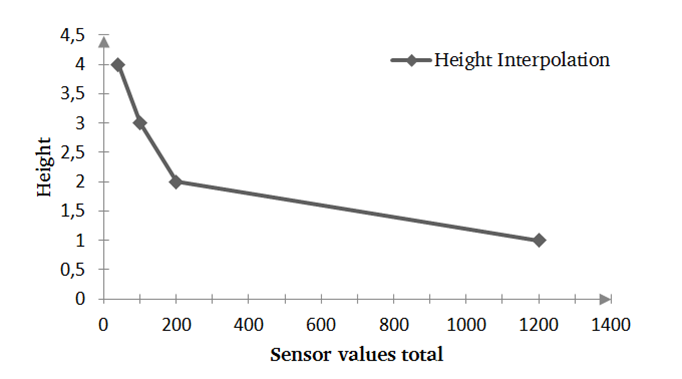
\includegraphics[width=0.6\textwidth]{images/magicbox_data_zaxis}
\caption{Piecewise linear hand distance estimation \cite{Braun2011MultiInputDevice}}
\label{fig:magicbox_data_zaxis}
\end{figure}
%Figure 29 Piecewise linear hand distance estimation [78]
The first data processing step of the MagicBox is the planar localization of the hand, following the weighted average algorithm previously presented. In order to calculate the distance of the hand from the plane we are using a piecewise linear interpolation, that resembles the response curve of a single sensor \cite{Braun2011MultiInputDevice}.
\begin{figure}[h]
\centering
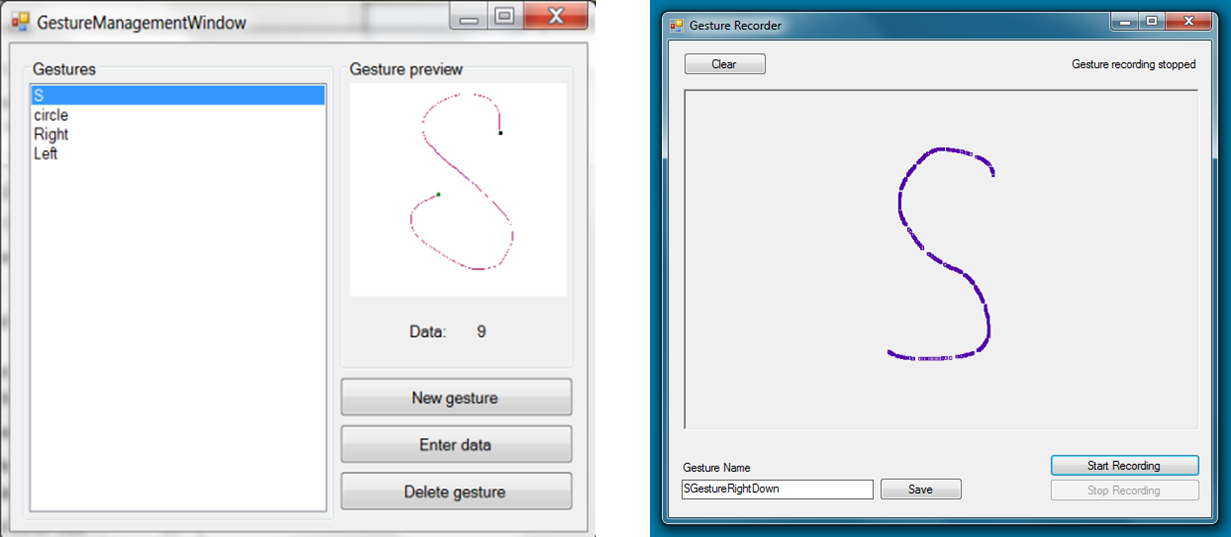
\includegraphics[width=0.7\textwidth]{images/magicbox_data_gest}
\caption{Gesture overview module (left) and gesture recorder (right)}
\label{fig:magicbox_data_gest}
\end{figure}
%Figure 30 Gesture overview module (left) and gesture recorder (right)
An addition of the MagicBox was a generic gesture recognition module based on methods similar to mouse gesture recognition \cite{braun2013capacitive}, albeit adapted for three dimensional locations. The developed debug software allows defining an arbitrary set of potential gestures and adding training data, as shown in Figure \ref{fig:magicbox_data_gest}. The module is looking for matches based on the most recent set of locations. 
\subsubsection{Large-area location tracking}
Using long wire electrodes may result in considerable noise and influence from outside electric fields. Therefore CapFloor requires preprocessing to reduce the noise and achieve a more robust high-level data processing. The localization uses the weighted average algorithm that has been presented previously. 
\begin{figure}[h]
\centering
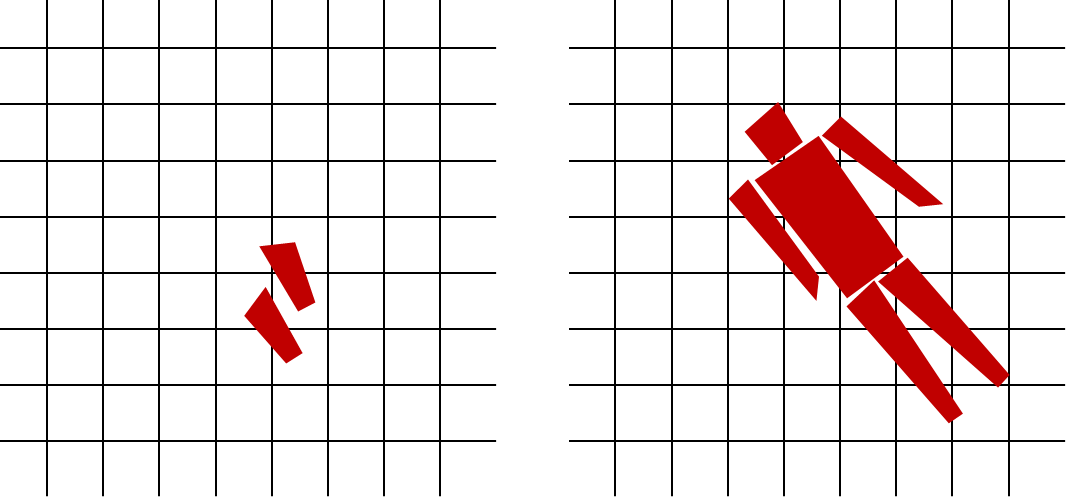
\includegraphics[width=0.8\textwidth]{images/floor_shapes}
\caption{Shapes of a standing and lynig person on top of the CapFloor grid}
\label{fig:capfloor_shapes}
\end{figure}
The fall detection is using a time-series analysis of the aggregated values of the sensors that are currently detecting an object. This method is using the assumption that the overall sensor response is roughly equivalent to the shape of the object that is closest to the surface, resulting in a higher capacitance of the overall system, similar to the plate capacitor model. This effect is shown in Figure \ref{fig:capfloor_shapes}. The sum $s$ of all n sensor values $r$ is the closest equivalent to the system capacitance and therefore a viable measure. If the overall value is beyond a certain threshold $v_l$ we can consider a lying person $p_l$.
\begin{equation}
s=\sum^n_{i=0}{r_i}\ \ \ ,\ \ \ p_l=\left\{ \begin{array}{c}
1,\ \ \ s\ge v_l \\ 
0,\ \ \ s<v_l \end{array}
\right.
\end{equation}
In order to increase the robustness this threshold has to be exceeded for a certain amount of time $t_m$. In consequence a fall $f$ is detected if the following equation is 1.
\begin{equation}
f=\prod^{t_m}_{j=0}{p_{l,t_j}}
\end{equation}
\subsection{Model-driven fitting methods}
\subsubsection{Single-body models}
\begin{figure}[h]
\centering
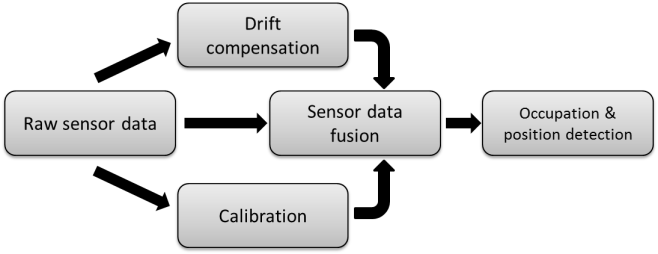
\includegraphics[width=0.7\textwidth]{images/smartbed_proc}
\caption{Data processing components \cite{braun2012context}}
\label{fig:smartbed_proc}
\end{figure}
The different components of the Smart Bed data processing are shown in Figure \ref{fig:smartbed_proc}. Raw sensor data is distributed to three different modules, the calibration which is determining the initial parameters for the sensor data fusion, the drift compensation that alters those parameters according to long term trends and finally the sensor data fusion module that processes the data and does feed it to the occupation \& position detection. Calibration and drift compensation follow the previously presented model \cite{braun2012context}. 
\begin{figure}[h]
\centering

\includegraphics[width=0.7\textwidth]{images/smartbed_cog}
\caption{Calculating centers of pressures and deviation \cite{braun2012context}}
\label{fig:smartbed_cog}
\end{figure}
Occupation and position detection is performed by dividing the two person bed into left and right and individually calculating for each side the total sensor values, assumed center of pressure using weighted average and the standard deviation (Figure \ref{fig:smartbed_cog}). The same calculation is done between the two sides to distinguish where is activity or if one person is lying diagonally.
Using these six intermediate values we can now map various poses. If all activity is on one side and the horizontal deviation is low, we can assume that one person is sitting. We can additionally use the intermediate values to calculate more information, e.g. the exact location a person is sitting at. 
The data processing for the sleep phase recognition is based on detecting the sensor data variations in order to analyze movement. Discriminating between sleep phases using movement is a common approach that has been used in the past \cite{salmi86}. Using a sparse set of sensors it is possible to detect movement by comparing subsequent sensor readings and associate it to different sleep phases using different activity profiles. The system is based on the same prototype as the posture recognition system \cite{Djakow2013movibed}.
\subsubsection{Multi-body models}
\begin{figure}[h]
\centering
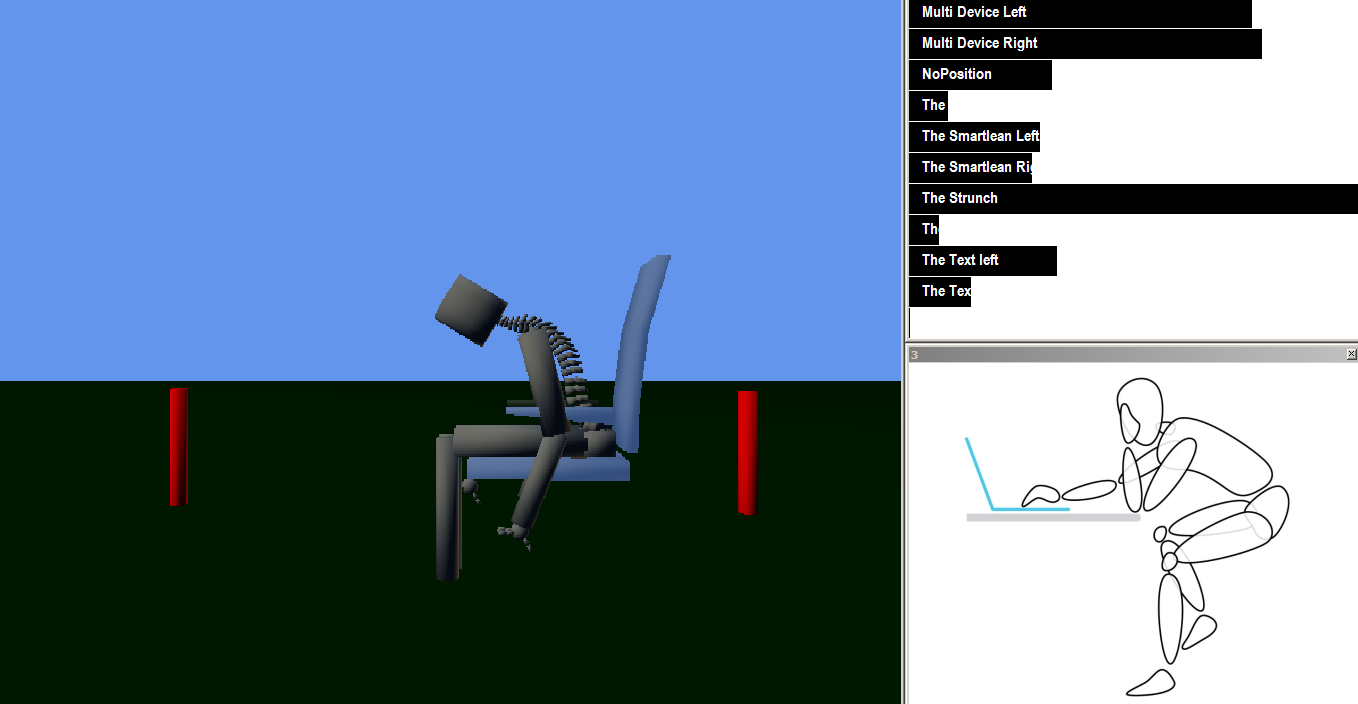
\includegraphics[width=0.7\textwidth]{images/smartchair_software}
\caption{Screenshot of the Capacitive Chair application showing the fitted 3D model on the left, posture detection on the upper right and the recognized posture on the lower right}
\label{fig:smartchair_software}
\end{figure}
In Figure \ref{fig:smartchair_software} we can see a screenshot of the Capacitive Chair debug application. On the left side we see a 3D model that is fitted to a chair model according to the current sensor values, in the middle the results of the machine learning module and the recognized posture and on the right side the currently running breathing rate detection as both Fourier analysis and signal deviation analysis.
All processing methods work on filtered and normalized sensor data. The difference in shape, material and size of the electrodes necessitates slight adaptations to noise filtering and data processing. As an example only the conductive thread backrest electrode is used in the breathing rate detection. 
The 3D model is using a simplified human joint model comprised of 13 connected components. Based on the current sensor readings, single parts or groups of components are fitted to the virtual chair. The process is a mix of posture mapping as found in the smart bed and modification of the dynamic links between the single components \cite{Braun2013ChairAid}.
\begin{figure}[h]
\centering
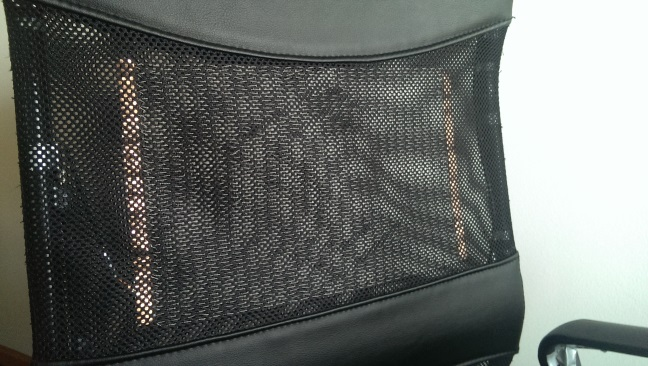
\includegraphics[width=0.7\textwidth]{images/smartchair_thread}
\caption{Screenshot of the Capacitive Chair application showing the fitted 3D model on the left, posture detection on the upper right and the recognized posture on the lower right}
\label{fig:smartchair_thread}
\end{figure}
We use a simple RBF neural network and training data collected by two different persons to match the input from eight sensors to nine potential output postures that are associated to different working situations. An early observation is that certain postures are difficult to distinguish given the limited number of sensors and the similarity of the postures on the rigid chair. Either a higher number of sensors or a more versatile chair could be used that allows gathering additional information required to distinguish the different poses more reliably. 

The breathing rate detection is operating on a single electrode that is integrated into a mesh on the backrest using conductive thread. The setup is shown in Figure \ref{fig:smartchair_thread}. Consequently the surface of the electrode is large and able to pick up the chest movement. Two different methods of data processing are used and fused to get the final breathing rate. Using a fast Fourier transformation the signal is transformed into the frequency space. We are looking for significant signal portions in frequency areas that can be associated to breathing, between $0.2Hz$ and $10Hz$. The second method is to look for zero-crossings of the sensor signal through an adaptive baseline. If a person is breathing in the sensor value will decrease resulting in the signal dropping below the long-term average, and rise above when the person is breathing out. Accordingly the breathing rate can be calculated by counting the zero-crossings.
\subsection{Heterogeneous sensor systems}
\subsubsection{Heterogeneous capacitive arrays}
\begin{figure}[h]
\centering
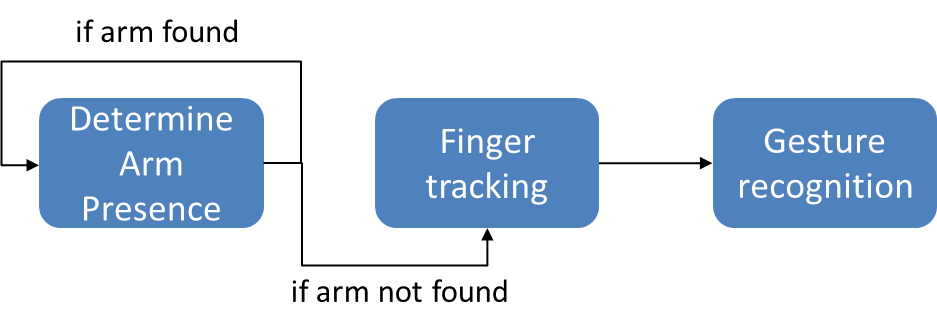
\includegraphics[width=0.4\textwidth]{images/armrest_dataproc}
\caption{Data processing pipeline of Active Armrest}
\label{fig:armrest_dataproc}
\end{figure}
%Figure 25 Data processing pipeline of Active Armrest
As we already mentioned, the Active Armrest electrodes are put into two groups. The data processing for both groups is distinctly different. In order to detect the presence of the arm using the two-electrode group a simple threshold on the accumulated values is used. The six sensor array in the front (touch area) is using the presented weighted average method to calculate finger positions. Additionally a threshold is used to distinguish one and two fingers. Overall there is a data processing pipeline as shown in Figure \ref{fig:armrest_proto}. The finger tracking and gesture recognition will be inactive until it is ensured that no arm is present. 

\subsubsection{Heterogeneous sensor fusion}
\begin{figure}[h]
\centering
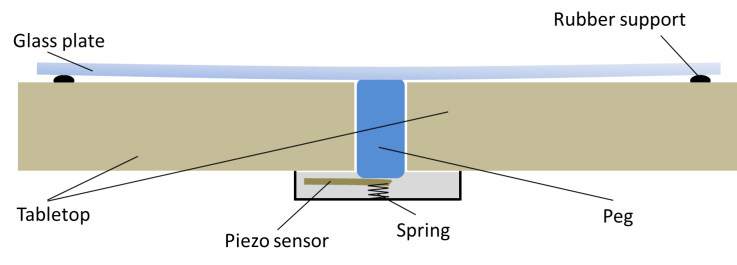
\includegraphics[width=0.7\textwidth]{images/captap_peg}
\caption{Suspended peg knock detection system for CapTap \cite{Braun2013ChairAid}}
\label{fig:captap_peg}
\end{figure}
%Figure 34 Suspended peg knock detection system for CapTap [80]
The hand location of the CapTap is similar to the methods presented for the MagicBox. We add the additional component of knock detection to provide selection events when touching the surface. Figure \ref{fig:captap_sketch} shows a sketch of the knock detection system. The table has a glass plate that is suspended on some rubber supports. In the center of the table we attach a small peg (enlarged in sketch) that creates a connection between the glass plate and a piezo sensor. If the glass plate starts vibrating from a touch we can measure this using the piezo sensor \cite{Braun2013ChairAid}. If a notable vibration is measured we are collecting the next 50 samples, resulting in a window of 250 milliseconds. To distinguish single and double knocks we calculate the weighted average within this window to get a measure for the distribution of sensor values within. If the average is closer to the beginning of the window the resulting event should be a single knock, and a double if the average is closer to the end of the window.
Hand localization and knock detection are working independently and are combined later in the software. It is reasonable to combine this, e.g. to ignore knock events that are occurring without a hand present. They may be indicative of a person doing a strong step close to the table.

\subsection{Image-based processing}
Their ability to detect changes in the electric field over a distance has led to capacitive proximity being regarded as similar to cameras. Smith et al. consequently called their approach electric field imaging, as particularly shunt mode measurements and their constrained electric fields allow applying certain image processing methods, e.g. tomography \cite{Smith1999a}. They were critical of using similar methods for shunt mode, noting the following statement.
\begin{quote}
Loading mode measurements can be likened
to images formed without a lens, since only one "end" of
each field line is constrained by the measurement. \cite{smith1998electric}
\end{quote}
Nonetheless, loading mode has certain advantages, particularly if all electrodes are in a single plane and we would like to have a higher sensitivity at a distance from the plane it is advantageous if there is no receiving potential nearby. One example for this planar electrode setup is large area gesture interaction devices, e.g. a table that is able to track the position of arms and hands in three dimensions. There is a plethora of image-based object detection and tracking algorithms that can be also used for capacitive proximity sensor data processing. There is a short process that I propose to realize this arm and hand tracking that includes some general steps that can be used to identify a variety of objects. The process is distinguished into four distinct steps:
\begin{itemize}
\item Creating a grayscale image from the acquired sensor data
\item Apply a feature-preserving image upscaling method
\item Find the contours of the present objects according to pixel values
\item Analyze the image moments of the contour areas and fit human arms
\end{itemize} 

\begin{figure}[h]
\centering

\includegraphics[width=0.5\textwidth]{images/proc_im_pixels}
\caption{Pixel array mapped from sensor values}
\label{fig:proc_im_pixels}
\end{figure}

The most challenging aspect of the first step is the low resolution of a reconstructed image. In order to achieve a mid-range distance resolution that allows detecting objects within 30 or 40 cm it is necessary to use electrodes that are sufficiently large. Thus, an example device uses an array of 6x4 sensor electrodes, resulting in an image of only 24 pixels. Typically the sensor values are an integer value in a range between 0 and 15000. Accordingly we can create a single-channel image with a channel depth of two bytes. In our case we use a linear mapping of sensor values to pixel intensities. An exemplary result image of this mapping is shown in \ref{fig:proc_im_pixels} (with enlarged pixels). In this format it is difficult to gather information about the exact position of the arms and thus we need to apply further processing before finding the contours and fitting arm objects.
\begin{figure}[h]
\centering
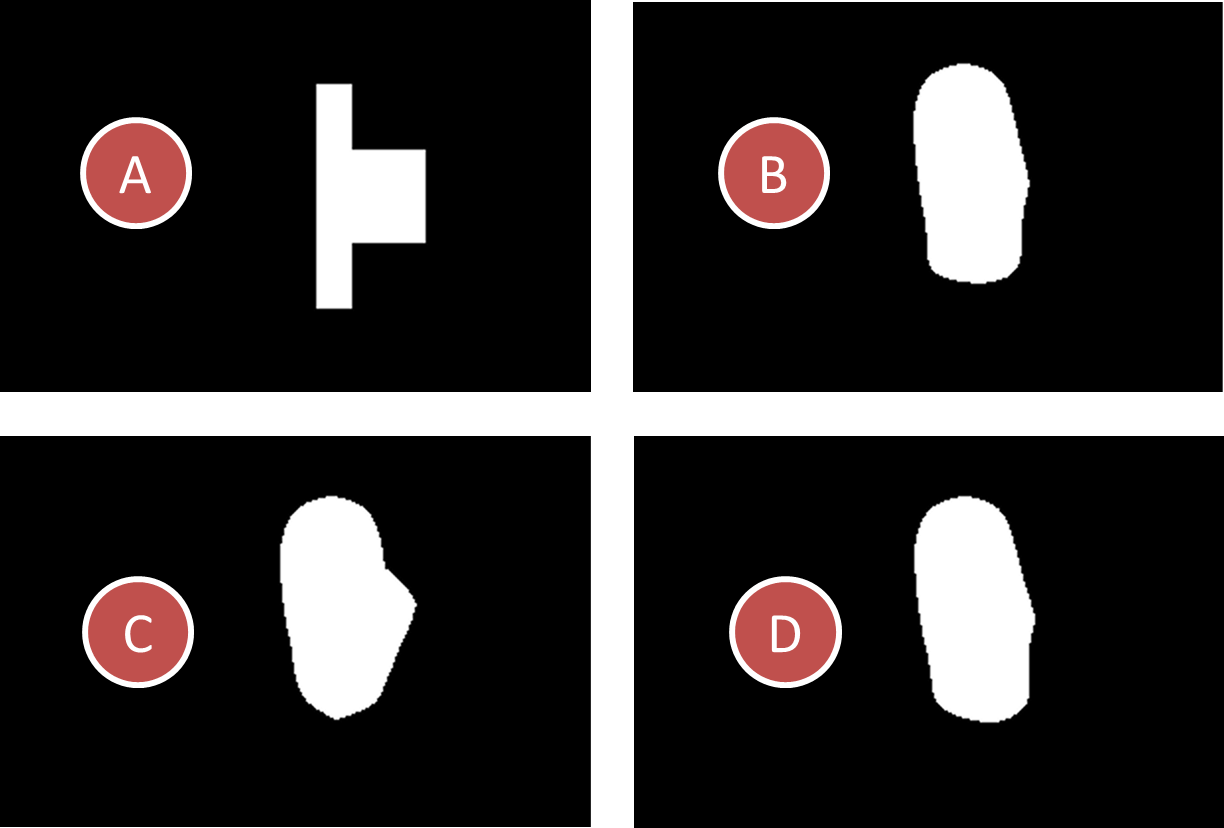
\includegraphics[width=0.9\textwidth]{images/proc_im_interpol}
\caption{Effect of different upscaling methods on shape, (A) nearest neighbor, (B) bicubic, (C) bilinear, (D) Lanczos4 - shown as thresholded binary images (pixel intensity > 30)}
\label{fig:proc_im_interpol}
\end{figure}

\subsubsection{Acquire and optimize contours}
In order to get the relevant contours of objects in the interaction area we have to apply some further processing. The first step is to enlarge the image using a feature-preserving scaling method. As all sensors are prone to environmental noise we apply some thresholding based on the pixel intensities before looking for contours. The result is an enlarged binary image of black and white pixels. We have tested four different image scaling methods, nearest neighbor, bilinear interpolation, bicubic interpolation and Lanczos interpolation. Exemplary results are shown in \ref{fig:proc_im_interpol}. The Lanczos interpolation showed the best results but is most processing intensive. However, since we are dealing with small images it is reasonable for CapTap. The contours are calculated based on those binary images, defined as the borders between black and white regions. For further processing we are looking into the distribution and the intensities of the pixels within the specified region.
\begin{figure}[h]
\centering
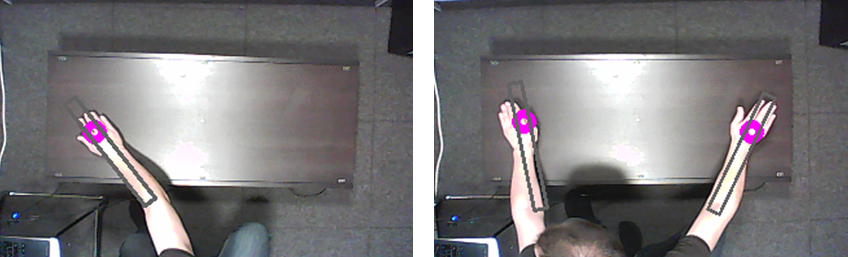
\includegraphics[width=0.9\textwidth]{images/proc_im_arms}
\caption{Overhead camera picture of the scene overlaid with live arm and palm reconstruction for one arm (left) and two arms (right)}
\label{fig:proc_im_arms}
\end{figure}

\subsubsection{Palm and arm fitting}
The last step of identifying and tracking the arms is to fit the position and orientation of the palms and arm into the acquired object contours. For this task we are analyzing the image moments within the contours. These are certain particular weighted averages of pixel intensities, or a function thereof \cite{hu1962visual}. They can be calculated using the following equation, whereas $j$ and $i$ define the order and $I(x,y)$ is the pixel intensity at a given position. We can use this to calculate the center point $(\overline{x},\overline{y})$, leading to the central moments $mu_ji$ that are required to determine the orientation of the contour as angle $\gamma$.
%m_ji=∑_(x,y)▒〖I(x,y) x^j y^i  〗,x ̅=m_10/m_00 ,y ̅=m_01/m_00 
%〖mu〗_ji=∑_(x,y)▒〖I(x,y) (x-x ̅ )^j (y-y ̅ )^i  〗
% γ=0.5∙arctan (2∙〖mu〗_11)/(〖mu〗_20-〖mu〗_02 )
\begin{equation}
m_ji=\sum_{(x,y)}{I(x,y)x^jy^i}
\end{equation}
\begin{equation}
\overline{x}=\frac{m_10}{m_00}, \overline{y}=\frac{m_01}{m_00}
\end{equation}
\begin{equation}
mu_{ji}=\sum_{(x,y)}{I(x,y)(x-\overline{x})^j(y-\overline{y})^i}
\end{equation}
\begin{equation}
\gamma=0.5\cdot arctan\frac{2\cdot{mu_{11}}}{mu_{20}-mu_{02}}
\end{equation}
 
We use the center point and orientation to calculate the estimated position of the palm of the hands. These points are the basis for the subsequent gesture recognition. Additionally, we are using separate Kalman filters for smoothing the different palm positions and arm orientation. The resulting arm reconstruction and the actual arm position in a photo are shown in \ref{fig:proc_im_arms}. We installed a simple webcam above the table and registered the table position to the camera image. 

The arm reconstruction so far is mostly used to determine the arm position. Another potential use of the arm orientation is to improve the merging of two hands. While the system can't distinguish from a single sensor if one hand is close or two hands are further away, we can use the presence of two arms to identify the overall number of objects in the detection range. 
\subsubsection{Intensity-based elevation estimate}
A distinct challenge of the capacitive hand tracking is the considerable directional difference in available resolution. While we can use the presented image analysis to track the planar position of the arms over the whole table area of 80cm width and 50cm depth, estimating the elevation of the arm above the table is restricted by the proximity range of the single sensor. Typically the achievable range maxes out at around 35cm, depending on environmental conditions. In a plate capacitor system the distance $d$ is proportional according to size of the plates $A$ and resulting capacitance $C$. Due to the linear mapping of sensor capacitance measurements to pixel intensities $I$ we can use the image moment within a contour $S$ as estimate of the actual capacitance, and calculate the elevation $e$ according to the following equations:

\begin{align}
d&\propto{\tfrac{C}{A}} & S&\propto{\tfrac{m_{00}}{\int{S}}}
\end{align}

The same thresholds discussed in the contour retrieval phase apply to this step, thus leading to discarding objects at a larger distance that are difficult to detect. Starting from this threshold we normalize the resulting elevation according to a maximum threshold for m00 that denotes a very close object (such as touch). The actual touch recognition is performed using acoustic methods. 
As previously explained the sensors are prone to environmental influences, thus this just allows to get an estimate of the actual elevation and no absolute distance value. Therefore, the interaction should not be designed to require a highly precise discrimination of different elevation values, but instead use more of a 2.5D paradigm. Our take on this will be presented in the application section.

\subsection{Physiological signals in frequency- and time-domain}

\clearpage
\section{Application prototypes}
\subsection{CapFloor}
\begin{figure}[h]
\centering
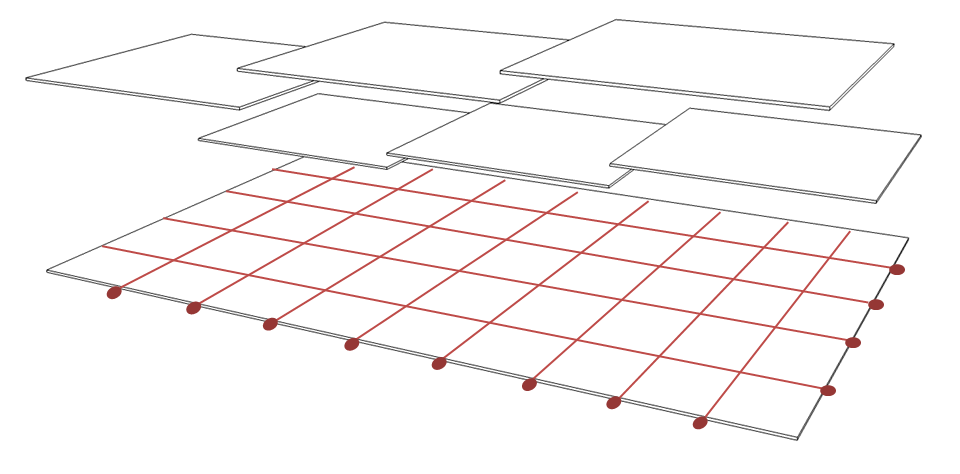
\includegraphics[width=0.8\textwidth]{images/capfloor}
\caption{CapFloor sketch - grid layout of electrodes is placed below a floor layer with sensors attached on the sides}
\label{fig:capfloor_sketch}
\end{figure}

CapFloor is a capacitive system for indoor localization and fall detection that is based on a grid array of sensing electrodes placed below a floor covering \cite{Braun2012CapFloor}. A sketch of the system is shown in Figure \ref{fig:capfloor_sketch}. The grid is comprised of insulated wires that are placed orthogonal to each other. Sensors are placed on two sides of the room. Each sensor is performing loading mode measurements. The system is intended to act as both indoor localization system and fall detector. CapFloor can be placed below any non-conductive material, like wood, tiles and PVC, if the distance between the wires and the floor surface is not too high. It can discriminate between a foot being above an electrode or a whole body. Combining this information from various sensors we are able to get a reliable detection of lying, sitting and standing persons. Using only two sides of the room for sensors it is possible to cut the wires without considerably affecting the signal; allowing easy installation in non-rectangular rooms.
Accordingly CapFloor is able to be used in various application scenarios. Indoor Localization in the home domain can be useful in energy saving and fall prevention by appropriately activating and deactivating the environment lighting. It can also be used in security-restricted areas to detect unauthorized movement. The fall detection should be used in a system that has various levels of escalation. E.g. it is not easy to distinguish between a person doing exercises on a floor and a person that has fallen down. Accordingly the system should query if the person is well and not autonomously call for outside help.

\subsubsection{Evaluation}
\begin{figure}[h]
\centering
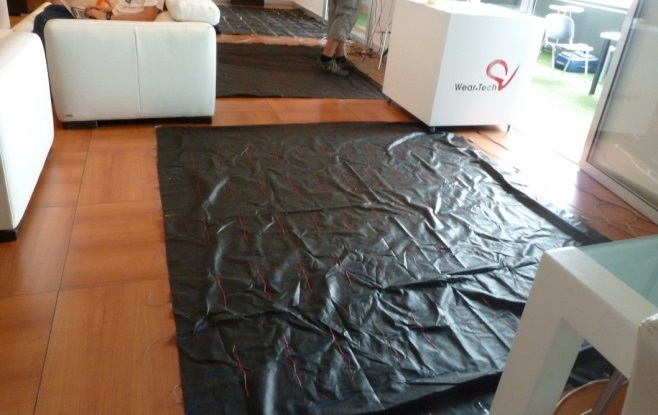
\includegraphics[width=0.8\textwidth]{images/capfloor_evaal}
\caption{Floor mats with integrated CapFloor system used at the EvAAL 2011 competition \cite{Braun2012CapFloor}}
\label{fig:capfloor_evaal}
\end{figure}
The CapFloor system was evaluated in the scope of the Indoor Localization Track of EvAAL 2011, where it participated out of competition \cite{chessa_eval}. In Figure \ref{fig:capfloor_evaal} we can see a picture of the demonstration setup installed in the living lap using the system integrated into different mats that are placed in the environment. The system was tuned to detect a single person and was able to perform this reasonably in the areas covered. The resolution of the system is strongly depending on the given density of electrode wires. While there is a certain measure of proximity, it is not possible to detect objects that are more than a few centimeters away from the wires. Later iterations of the system are using higher voltages and shunt mode measurements to improve the tracking reliability and enhance the fall detection.

\clearpage
\subsection{Smart Bed}
\begin{figure}[h]
\centering
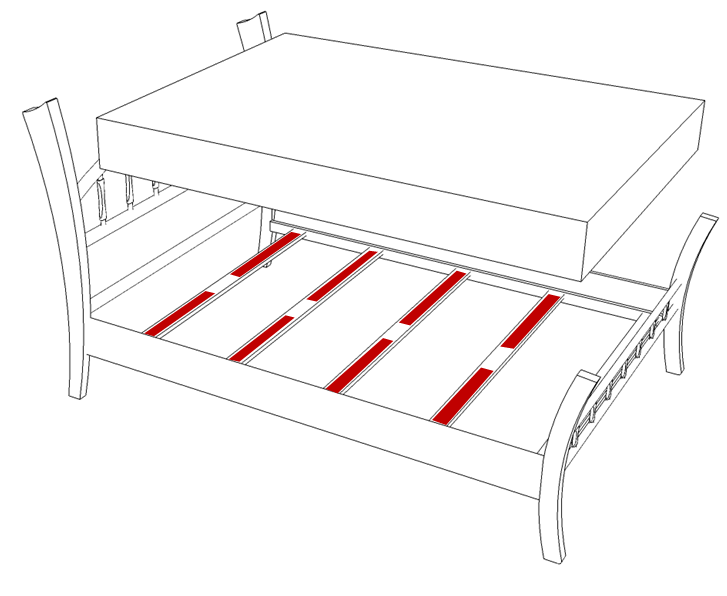
\includegraphics[width=0.7\textwidth]{images/smartbed}
\caption{Smart Bed sketch - flexible plate electrode are attached on spring board}
\label{fig:smartbed_sketch}
\end{figure}
The Smart Bed is a regular bed frame that has been equipped with capacitive proximity sensors in order to determine occupation, posture and sleep phases \cite{braun2012context}\cite{Djakow2013movibed}. A sketch can be seen in Figure \ref{fig:smartbed_sketch}.  The electrodes are comprised of copper foil that is attached to the flexible wooden panels of the slatted frame. This allows the electrodes to be sensitive to both proximity and applied pressure, resulting in a superposed combined sensor value that is considerably higher as opposed to proximity measure on its own. The electrodes are equally distributed, with four being on both sides of the two person bed. The system is able to determine different sitting and lying postures of one or two persons, including less regular lying positions such as diagonal or orthogonal to the long side of the bed. Using an analysis of the movement gathered by variation in the sensor signal the sleep phases can be analyzed, similar to accelerometer-based systems that are popular for smartphones \cite{krejcar2011}.

The Smart Bed can be used for various purposes. A main application is connecting the occupation detection to a home automation system and timer in order to activate ambient lighting if the person is get-ting up in the night, presumably to find the way to the restroom. Accordingly, in a single person household the lights in unoccupied rooms could be turned off in order to conserve energy. In the domain of personal health the Smart Bed is able to give the user a feedback on sleep quality based on the sleep phase measurement performed in the night. Another potential application is to use the acquired pressure distribution as indicator for back-friendly lying positions that may be harmful over a longer period of time \cite{Hamisu2010}.
The occupation and posture detection relies on a simplified body model to approximate the pressure distribution and sensor values to a certain posture \cite{braun2012context}.  

\begin{minipage}{\linewidth}
\centering
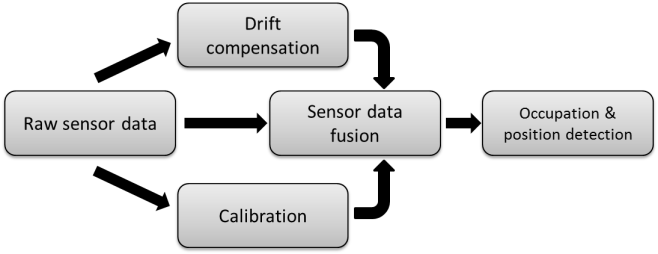
\includegraphics[width=0.7\textwidth]{images/smartbed_proc}
\captionof{figure}{Data processing components \cite{braun2012context}}
\label{fig:smartbed_proc}
\end{minipage}

The different components of the Smart Bed data processing are shown in Figure \ref{fig:smartbed_proc}. Raw sensor data is distributed to three different modules, the calibration which is determining the initial parameters for the sensor data fusion, the drift compensation that alters those parameters according to long term trends and finally the sensor data fusion module that processes the data and does feed it to the occupation \& position detection. Calibration and drift compensation follow the previously presented model \cite{braun2012context}. 

\begin{minipage}{\linewidth}
\centering
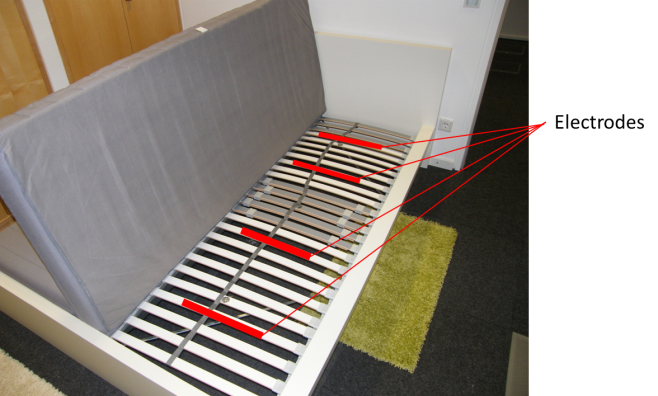
\includegraphics[width=0.8\textwidth]{images/disc_unob_bed}
\captionof{figure}{Electrodes and sensors hidden below mattress of Smart Bed \cite{braun2012context}}
\label{fig:disc_unob_elec}
\end{minipage}

The system prototype is shown in Figure \ref{fig:disc_unob_bed}. The positions of the electrodes on the slatted frame are indicated in red. The picture only shows one side of the bed. The same electrode positions are used on the other half of the bed.

The data processing for the sleep phase recognition is based on detecting the sensor data variations in order to analyze movement. Discriminating between sleep phases using movement is a common approach that has been used in the past \cite{salmi86}. Using a sparse set of sensors it is possible to detect movement by comparing subsequent sensor readings and associate it to different sleep phases using different activity profiles. The system is based on the same prototype as the posture recognition system \cite{Djakow2013movibed}.
 
\subsubsection{Evaluation}
\begin{figure}[h]
\centering
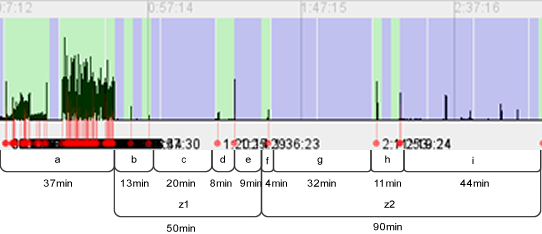
\includegraphics[width=0.9\textwidth]{images/smartbed_sleepphase}
\caption{Sleep movement data over three hours in one night \cite{Djakow2013movibed}}
\label{fig:smartbed_sleepphase}
\end{figure}
The Smart Bed posture recognition is able to successfully distinguish eight typical sitting and lying states. Using adaptation of the intermediate values it is possible to fit the state to an actual position on the bed, e.g. a \emph{person sitting on the right side of the bed} state can be modified to any location on that specific side of the bed. 
Regarding the detection of sleep phases there has been an evaluation and benchmarking of three nights \cite{Djakow2013movibed}. The Smart Bed was able to achieve a comparable performance to smartphone applications that detect sleep phases based on accelerometers. Figure \ref{fig:smartbed_sleepphase} gives an example of movement recordings using the capacitive proximity sensors over one night. The activities are grouped into distinct chunks that are later associated to the sleep phases. Currently breathing rate detection is added to the Smart Bed that can be used to improve the sleep phase detection and also can potentially detect anomalies that may be indicative of a certain health risk.

\clearpage
\subsection{The Capacitive Chair}
\begin{figure}[h]
\centering
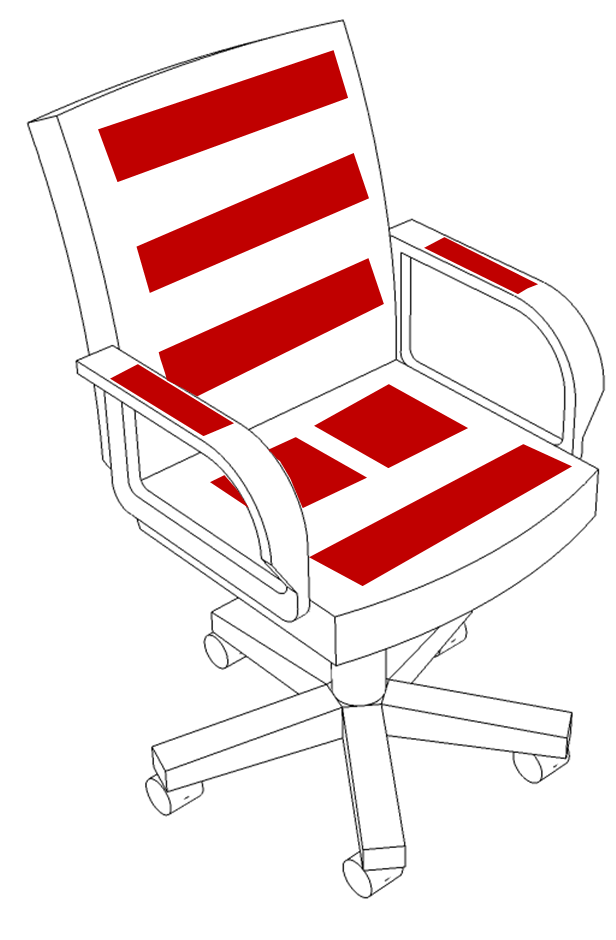
\includegraphics[width=0.4\textwidth]{images/smartofficechair}
\caption{Smart office chair sketch - eight electrodes three in backrest, three on seat and two in armrests}
\label{fig:smartchair_sketch}
\end{figure}
The Capacitive Chair is a regular office chair equipped with eight capacitive proximity sensors that can detect different sitting postures and work-related stress levels by examining movement and breathing rate \cite{Braun2013ChairAid}. Seven solid copper electrodes that are placed below the covering are augmented by a single conductive thread electrode that is placed in a mesh on the backrest. In the past smart chairs have used pressure sensors to infer posture and occupation \cite{tan2001sensing}. Combining presence and proximity sensing it is possible to directly infer postures where parts of the body do not touch the surface, e.g. if the body is arched towards the front, or if an arm is raised from the armrests. Additionally higher area electrodes in the backrest allow detecting the breathing rate by measuring the movement of the chest.

The Capacitive Chair aims at providing different services to a typical office worker and office managers. Using the occupation detection it is possible to advise for some type of physical activity, if the time spent in front of the screen was too long. The system can also advise the user to change to a more back-friendly posture or regularly switch the stance to achieve a more general workout. Using the breathing rate detection we are able to get some sort of measure of the current stress level associated to the given working situation. By adapting the environment it is possible to improve the working atmosphere and reduce stress. The Capacitive Chair uses a multifacetted data processing approach. A machine learning algorithm is associating the sensing data to one of nine different typical sitting positions, inspired by a recent study of sitting positions for modern device usage \cite{globalPosture}. An adaptive body model that is fitted to the current sensor values allows for fine grained adaptation of those postures. Finally a combination of Fourier and data variation analysis is calculating the current breathing rate \cite{Braun2013ChairAid}.

\subsubsection{Capacitive layout}
The Capacitive Chair is based on a single OpenCapSense board that supports eight different electrodes. In order to get the posture measurements we need to distribute the electrodes equally on the different areas of the seat. The measurement of the breathing rate requires a larger electrode near the chest area. Consequently the electrodes are placed as follows:
\begin{enumerate}
\item Electrode on the upper part of the backrest (covered by faux leather)
\item Electrode in the central part of the backrest (using conductive thread)
\item Electrode in the lower part of the backrest (covered by faux leather)
\item Electrode below the right armrest
\item Electrode below the left armrest
\item Electrode for the left hip area below the left part of the seat
\item Electrode for the right hip area below the right part of the seat
\item Electrode for detecting both legs below the front part of the seat
\end{enumerate}

\begin{minipage}{\linewidth}
\centering
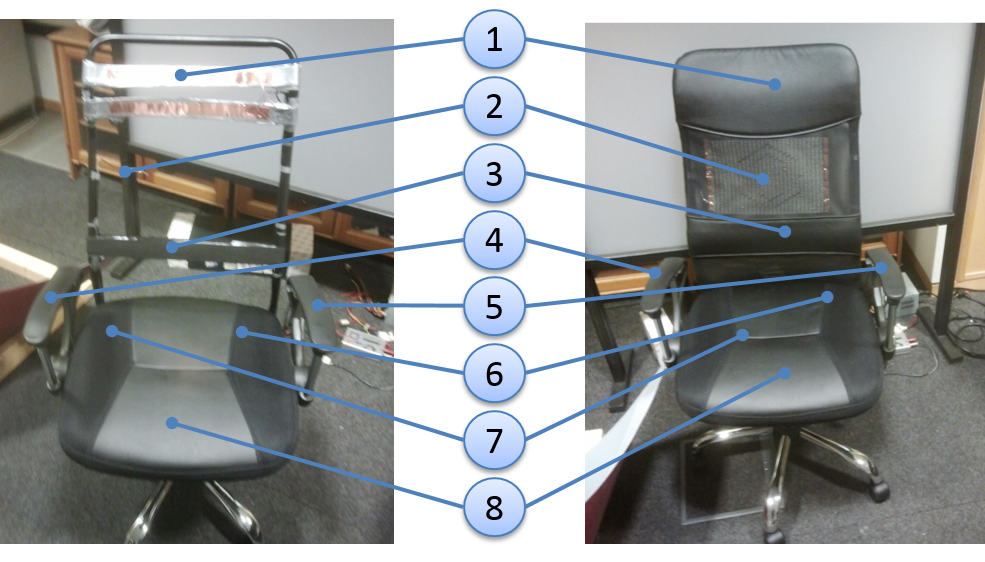
\includegraphics[width=0.8\textwidth]{images/prot_capchair_electrode_layout}
\captionof{figure}{Capacitive Chair electrode positions}
\label{fig:prot_capchair_electrode_layout}
\end{minipage}

The electrode is connected to channel 0 (CH0) of the OpenCapSense evaluation board. The following figure shows the layout of the electrode (2) including sensing electronics (5). The shield electrode is additionally the support structure for the whole setup here. The shield electrode is comprised of copper sheet bedded in duct tape. On the duct tape there are strips of copper sheet applied using conductive glue (2). The copper sheet is the sensing electrode connected to the sensor (5) using the blue wire (4). The shield electrode is connected using the red wire. The frame of the backrest is indicated using the number (6). 
This electrode in the lower part of the backrest is connected to CH2 of the OpenCapSense evaluation board.
The layout is analog to the one on the upper part of the backrest, comprised of shield electrode (2) covered by duct tape and a copper sheet electrode. The electrode on the right armrest is connected to CH3, the one on the left side to CH4 of the OpenCapSense evaluation board. Both electrodes are comprised of a copper sheet fixed to the armrest using duct tape. 
The electrode below the right hip area is connected to CH5, the one below the left hip area to CH6 and the leg electrode to CH7.
The figure above shows the electrodes. All of them are made of unprocessed, two-layer copper PCBs. They are isolated to the environment using duct tape. The electrode for the leg area is comprised of two distinct PCBs (2,3) that are connected using copper wire (5). The hip electrodes (1) are similarly comprised of copper PCBs. The wires are guided through the wooden seat using small drill holes (4,6). The red wire leads to the sensing electrode while the grey wire leads to the shielding.

\begin{minipage}{\linewidth}
\centering
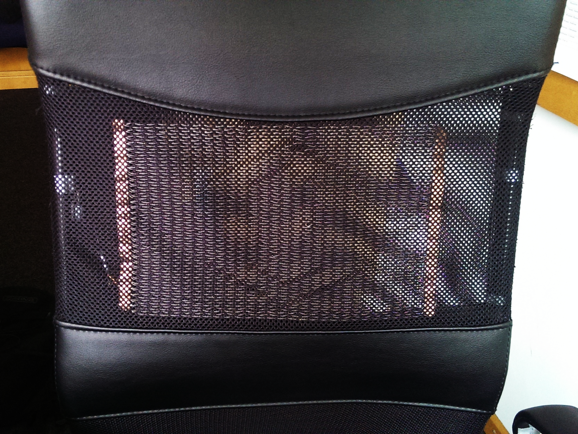
\includegraphics[width=0.8\textwidth]{images/prot_capchair_threadelectrode}
\captionof{figure}{Detail view of conductive thread electrode}
\label{fig:prot_capchair_threadelectrode}
\end{minipage}

The electrode in the central part of the backrest is connected to CH1 of the OpenCapsense evaluation board.
The electrode (1) is comprised of conductive thread that was woven into the covering of the backrest. The ends of the conductive thread are connected to a conductive copper foil. This foil is formed in such a way (4 left) that a terminal (4 right) can be applied and connected to the sensor electronics (3). This type of electrode does not support any shielding. In order to remove the covering the terminal should be disconnected from the electrode first.
 
\subsubsection{Processing}
The first step of data processing is filtering. We have implemented different types of filters, including static average and floating average filters. In this case we are using a median filter that is taking the median value of eight previous samples. After filtering we are building the baseline for each sensor channel. The baseline is the minimal sensor value that is created by sampling the environment without any object present. There is a plausibility check in this step to discard values that deviate too far from the norm. The maximum values of a channel are collected on run-time. Again we are using a plausibility check. The final step of pre-processing is a normalization based on acquired minimum and maximum values. For further processing we additionally need information about short-term value variance that we gather by calculating the difference quotient using a sample of ten average filtered measurements.
Afterwards we are performing a fast fourier transformation (FFT) to get information about the frequency spectrum of the sensor values, in order to perform breathing rate detection. 
\subsubsection*{Breathing rate detection} 
We are using the FFT values of sensors attached to the central backrest to get the current breathing rate. A binning operation is performed to look for significant signals in a reasonable frequency interval (0.1Hz-3Hz).
In order to increase the reliability of the breathing rate detection we use a second method. Based on the normalized values a mean value curve is calculated. The intersection points of this mean value curve and the current sensor values are additionally stored. We are using a dynamically weighted combination of both values to increase the reliability of the breathing rate detection.
\subsubsection*{Posture recognition, kinematics of the human body}
The processed values of all sensors are compared to previously trained sitting positions of a user. The position with the lowest deviation is considered the current posture. Currently the system supports nine different postures; however it can be dynamically extended or reduced.
Based on the normalized sensor values and geometric positions of the sensors the data is interpreted as position of the different joints of a user. 
4.2.4	Output
The GUI allows displaying of raw and processed data. In the following section we are presenting the different forms of interaction.
 
Figure 13 GUI with four opened windows
Figure 11 gives on overview of the GUI. Selecting the desired output in the ToolBox (1) opens the associated window. In this case we can see the data display of sensor channel 1 (2), the recognized breathing rate (4), the FFT of sensor channel 1 (3) and the recognized postures and their deviations (5).
 
Figure 14 GUI with two windows
Figure 12 shows two additional windows. On the left side (1) we can see a picture depicting the currently recognized posture; on the right side (2) we can see the human model with recognized joint positions. The 3D joint recognition is still in strong development and will be remodeled in the future.
Additional screens that have not been shown in this overview are a serial monitor that displays the raw data acquired from the USB connection, the collection of measurements using software queries, the display of all sensor values in table format and a repositioning of the different windows.
\subsubsection*{Distinguish work activity levels}
 
Figure 15 Work Activity aggregation over a single work day (mock-up)
Figure 13 shows a mock-up of a typical work day activity over a single work day. We assume the work day of a typical office worker and support three different aggregated activities: 
Active work as indicated by a certain level of movement while on the chair
Passive work as being present on the chair while not moving a lot
Not present at desk, whereas no one is currently sitting on the chair.


\subsubsection{Evaluation}
The Capacitive Chair was partially supported by the EIT ICT Labs project Cognitive Endurance during 2013. In this scope it was evaluated in two distinct studies. The first aimed at testing the aggregated recognition of working activities with several persons over various days. The second study was testing the posture recognition with various users that were additionally queried about their general impression of the system. In this section we are presenting results of both studies.
\subsubsection*{Working situation recognition}
The sensing chair supports distinguishing two different working situations that are determined using the method described in the previous section. The system also supports sending to the Cognitive Endurance server.
 
Figure \ref{fig:prot_capchair_eval_work} shows an example of this generated activity log. We have performed a test over 3 days between December 4th 2013 and December 6th 2013 on a typical work day in the office. The resulting activity logs were used to generate a chart as shown in the previous section. An example chart is shown in Figure 15.

\begin{minipage}{\linewidth}
\centering
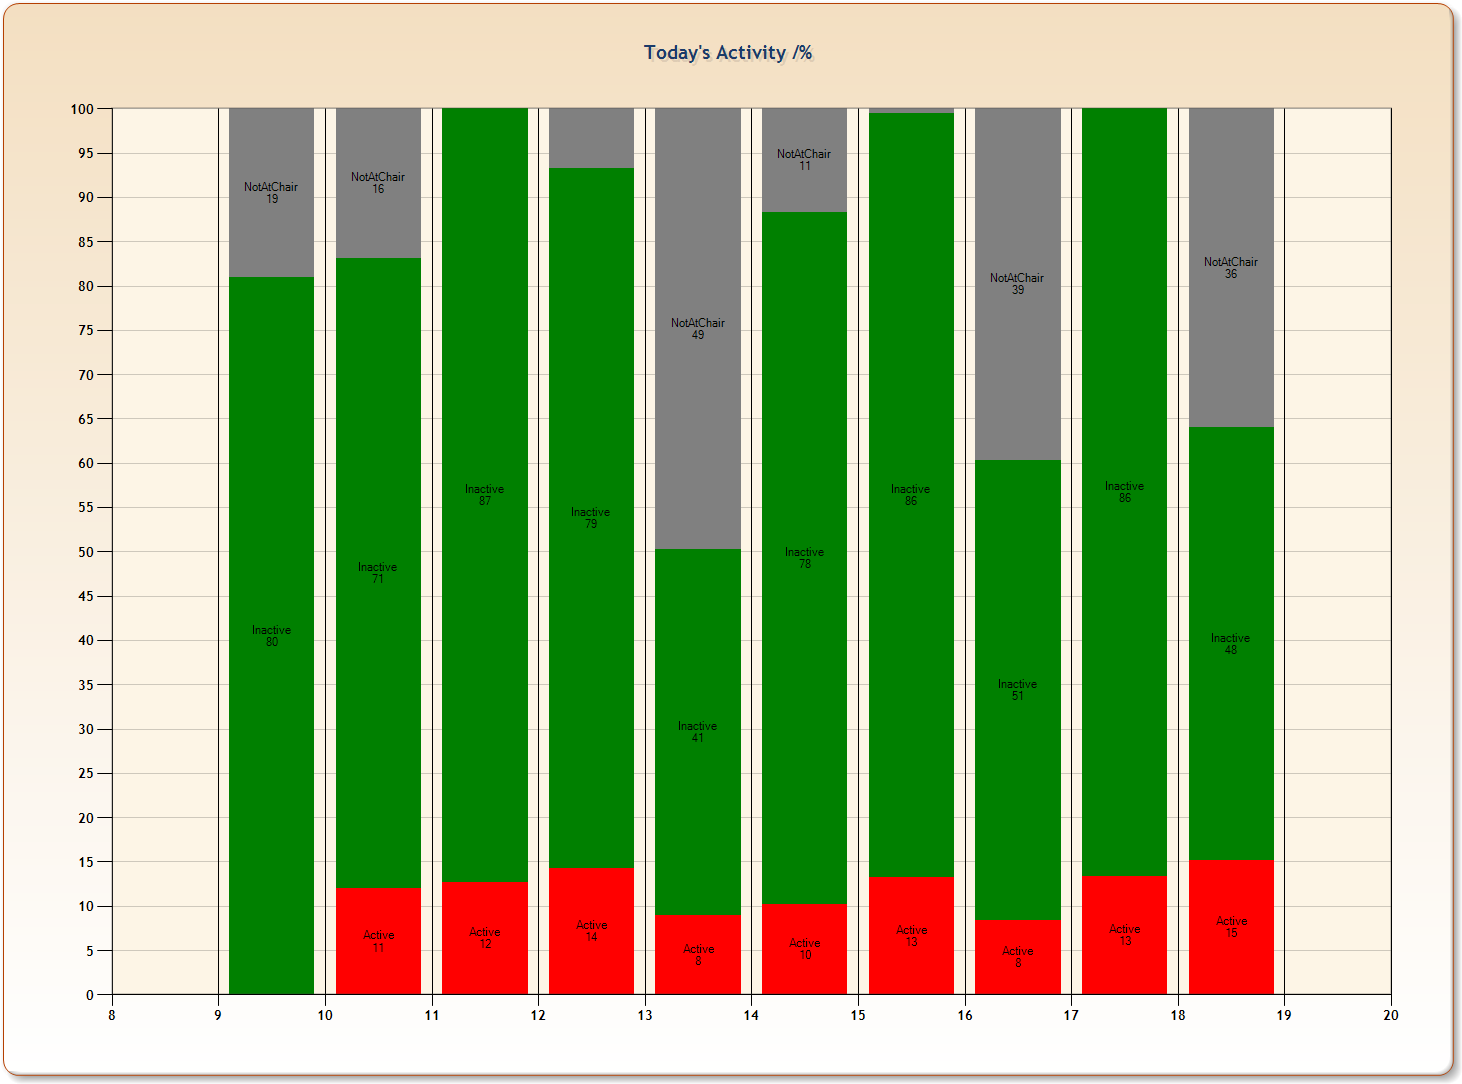
\includegraphics[width=0.8\textwidth]{images/prot_capchair_eval_work}
\captionof{figure}{Example chart of work activity data collected}
\label{fig:prot_capchair_eval_work}
\end{minipage}	

We can clearly see some phases of not at chair - usually for lunch break or some meetings and the work is distributed between active work, such as writing and typing and longer phases of inactivity (such as reading).

\subsubsection*{Posture recognition - test 1}
In a second evaluation we were testing the posture recognition of the chair in a short study with 10 participants. Our system was tuned to distinguish three poses and a non-pose:
\begin{itemize}
\item Sitting upright
\item Sitting hunched
\item “Slouching on chair”
\item Close to chair - disturber
\end{itemize}

The persons were given a short introduction, the different postures were displayed, and finally the persons were asked to perform the postures in order. When testing “close-to-chair” the subjects were asked to rattle at the chair, stand close, move it around and thus disturb the potential sensor readings. Each class was tested for 10 seconds, collecting 200 samples. Some impressions can be found in the following pictures:

\begin{minipage}{\linewidth}
\centering
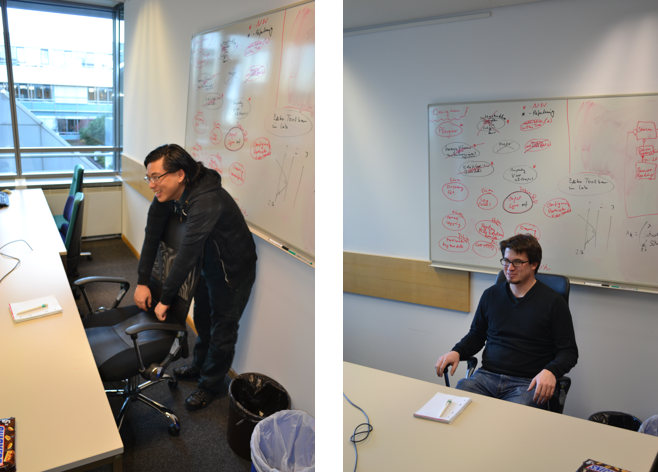
\includegraphics[width=0.8\textwidth]{images/prot_capchair_eval_pos1}
\captionof{figure}{Disturber position of a participant (left) and sitting upright (right)}
\label{fig:prot_capchair_eval_pos1}
\end{minipage}	 

\begin{minipage}{\linewidth}
\centering
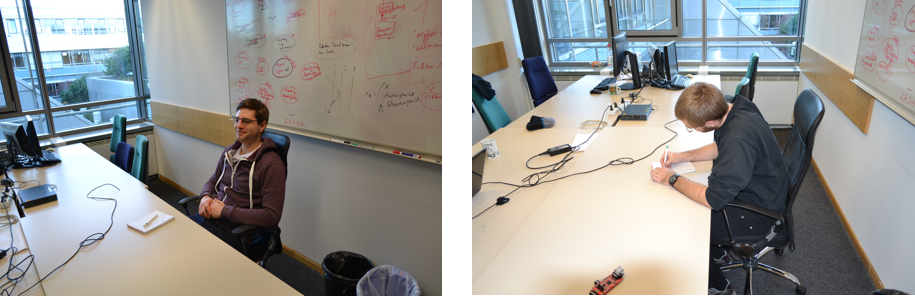
\includegraphics[width=0.8\textwidth]{images/prot_capchair_eval_pos2}
\captionof{figure}{Slouching position (left) and sitting hunched (right)}
\label{fig:prot_capchair_eval_pos2}
\end{minipage}

Overall the results were very convincing. Of the 40 different measurements series only two were not achieving 100\% accuracy. The Upright and Disturbance positions were classified correctly for all candidates. A single candidate had an 86\% rating on the hunched posture. A different candidate had a 55\% rating on the slouching position. The average of correctly classified postures is 98,5\%.



\clearpage
\subsection{Active Armrest}
\label{ch:prot_armrest}
\begin{figure}[ht]
\centering
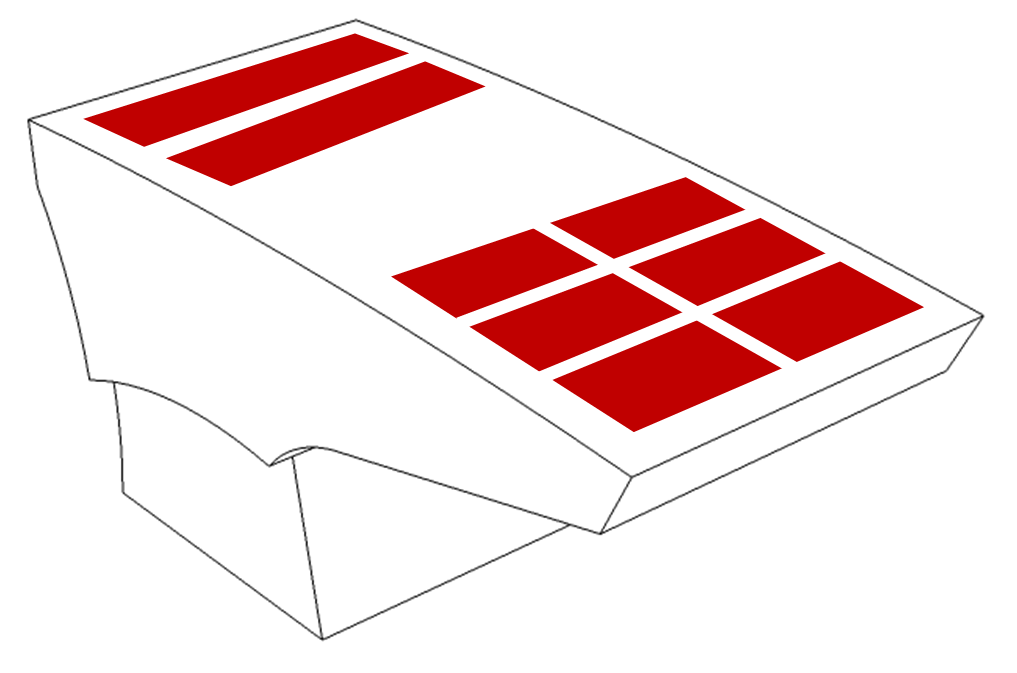
\includegraphics[width=0.4\textwidth]{images/active_armrest}
\caption{Active armrest sketch - six electrodes for finger gesture detection in front, two for arm detection in back}
\label{fig:armrest_sketch}
\end{figure}

Touch screens are by now also a trend in vehicles, with touch screens and touch pads becoming more common. The Tesla Model S provides a large area touch screen that completely replaces conventional button-based interfaces.  However, touchscreens have been identified as potentially distracting for the driver \cite{rumelin2013make}. My idea was to create a gesture input device based on capacitive proximity sensors, and unobtrusively integrate it into the car interior \cite{braun2013ActiveArmrest}. A suitable area for creating an interactive zone is the armrest, as it is the intended resting position in the first place. However, this creates an additional challenge. As the majority of interactions between arm and armrest are not intended to control aspects of the car system, we need concepts to infer the intention of the driver to interact with the car. The method has been described previously in Section \ref{ch:proc_hetero}. A sketch of this concept is shown in Figure \ref{fig:armrest_sketch}. To test the validity of the invisible interactive areas and the two interaction concepts, we have created the Active Armrest, a prototype comprised of an aftermarket armrest with an integrated heterogeneous array of eight capacitive proximity sensors - two using large electrodes for detecting arm proximity and orientation and six using small electrodes to create an interaction area in front of the armrest. The system uses the classification method described in Section \ref{ch:proc_hetero}.

\begin{figure}[ht]
\centering
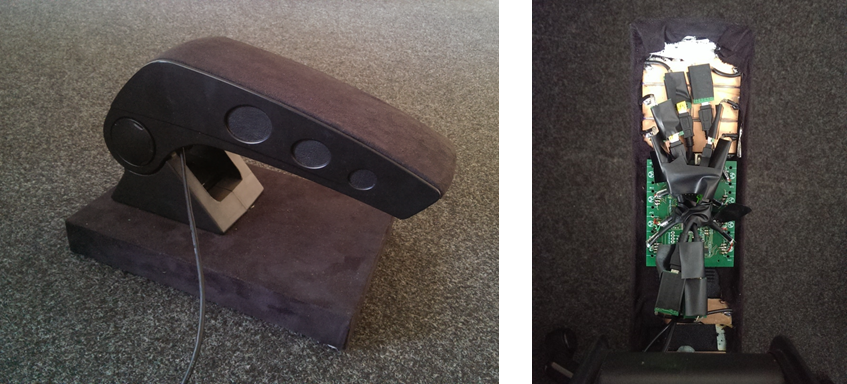
\includegraphics[width=0.8\textwidth]{images/armrest_proto}
\caption{Active Armrest prototype, left - outside view, right - detail view of electronics \cite{braun2013ActiveArmrest}.}
\label{fig:armrest_proto}
\end{figure}

In order to evaluate the Active Armrest we have built the prototype shown in Figure \ref{fig:armrest_proto}. An aftermarket armrest was equipped with an OpenCapSense toolkit. The kit had to be modified due to the constrained interior and uses fixed wiring instead of USB connections. The demonstration application is based on the SenseKit debug software supplied with the toolkit. As of now there is a simple USB connection to a nearby PC. The gesture recognition framework was implemented in Java using the WEKA machine learning framework for SVM classification. A car interior demonstration application was created using Java and the Swing framework and mimics typical menu systems found on a touch screen.

\begin{figure}[ht]
\centering
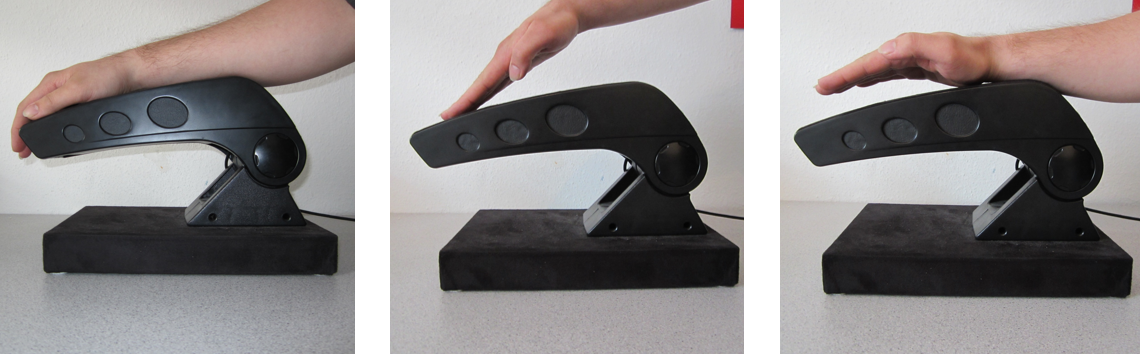
\includegraphics[width=0.8\textwidth]{images/armrest_postures}
\caption{Postures of limbs on armrest - resting position (left),  arm raised position (middle), hand raised position (right) \cite{braun2013ActiveArmrest}.}
\label{fig:armrest_postures}
\end{figure}

In Figure \ref{fig:armrest_postures} we can see the three different positions arm and hand can have on the armrest. On the left, arm and hand are in resting position with both close to the surface. The middle image shows the arm raised position and fingers touching the front of the armrest. The right picture shows the arm resting on the back and the hand in proximity of the front area. The system is able to distinguish between the three different positions using the methods presented in Section \ref{ch:proc_hetero}. A set of four different gestures has been defined for both interaction methods. The number is sufficient to control the user interface that was developed and supports both navigation and selection. The type of gestures has been defined after looking at previous research into touch and hand gestures \cite{bragdon2011experimental, wachs2011vision}. For the touch interaction, left and right swipes performed with either one or multiple fingers are supported. Regarding the free-air interaction we are using left and right swipes, as well as planar circles either clockwise or counter-clockwise.

\begin{figure}[ht]
\centering
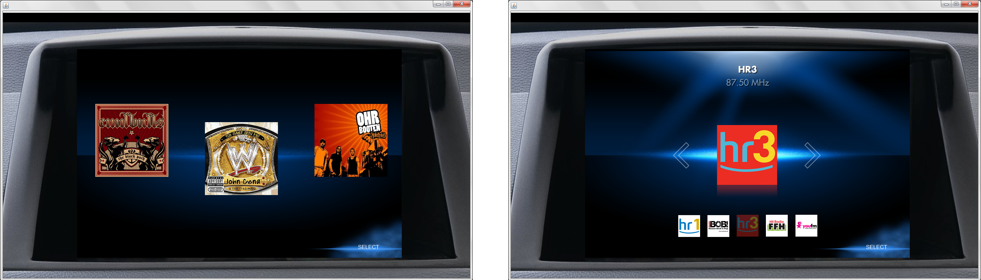
\includegraphics[width=0.8\textwidth]{images/armrest_demo_app}
\caption{Active Armrest demo software, left - finger tracker, right - OSM based navigation application \cite{braun2013ActiveArmrest}}
\label{fig:armrest_demo_app}
\end{figure}

Figure \ref{fig:armrest_demo_app} shows two screenshots of the created demonstration application. It allows to control radio stations, selecting different audio files and looking at images. It is controlled using the gesture sets explained above. The applications use a Next/Previous pattern for navigation within a UI level and Select/Back gestures to switch between the different levels of the UI.

\subsubsection{Evaluation}
\begin{figure}[ht]
\centering
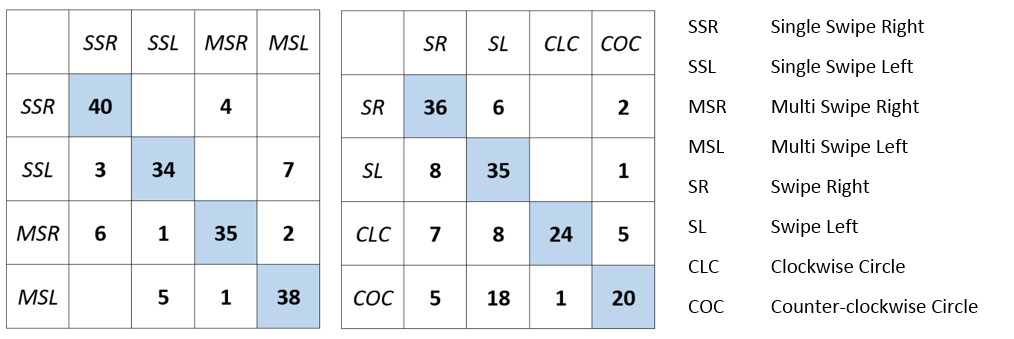
\includegraphics[width=0.8\textwidth]{images/armrest_eval_confustion}
\caption{Confusion matrices of recognized gestures for touch interaction (left) and free-air interaction (right)}
\label{fig:armrest_eval_confustion}
\end{figure}

We performed a study with 11 participants investigating three different aspects - the detection rate of the gesture recognition system, differences in interaction speed between the two methods and getting a general feedback on the usability of our system. After a short introduction, the participants were asked to perform each gesture 4 times for both sets in alternating starting order. The results are shown in Figure \ref{fig:armrest_eval_confustion}. The touch interaction performed reasonably with a detection rate between $79.5\%$ and $90.9\%$ for each gesture. The detection rates of the free-air interaction were considerably lower, ranging from $45.5\%$ for counter-clockwise circles to $81.8\%$ for swipes to the right. The main issue is distinguishing between single and multi-touches. A personalized threshold that is calibrated to the user might alleviate this issue in future iterations. The interaction zone above the finger area is limited to a range of about 15 cm. While performing the circular gestures the participants often left this area, leading to misattribution to swipe gestures.

In the second part of the evaluation the participants had to perform a task in the presented demonstration application - selecting and playing back a certain music file. We calculated the time required to perform the task. The average time for free-air gestures ($\mu=125.67s, \sigma=95.12s$) was considerably higher than the average task completion time for touch gestures ($\mu=34.26s, \sigma=28.61s$). It is noticeable that there is a very high deviation of the different runs, while the touch gestures fare better in general. While many users were able to quickly perform the task, others had a high number of errors and required several minutes. We can assume that a certain amount of training can reduce the required time. A trained user not participating in the study required 11 s for the touch gestures and 18 s for the free air gestures.

Finally, we asked the participants to fill a general questionnaire on their experience with the Active Armrest comprised of a number of Likert-scale (1-10) questions. There was a strong preference for the touch gestures, in line with the results of the interaction time and gesture recognition study (1=touch gestures, $\mu=1.72, \sigma=0.84$). Most participants could imagine using the system for a longer period of time in their cars (10=strong agree, $\mu=8.00, \sigma=2.00$) and considered the device intuitive to use (10=strong agree, $\mu=8.36, \sigma=1.67$) and is an interesting interaction device (10=strong agree, $\mu=8.63, \sigma=1.26$). The touch interaction pattern was considered easier to use (10=very easy, $\mu=8.00, \sigma=2.45$) than the free-air interaction (10=very easy, $\mu=3.64, \sigma=2.68$). The opinions on the device precision were mixed (10=very precise $\mu=7.27, \sigma=2.43$).


\clearpage
\subsection{Magic Box}
\begin{figure}[h]
\centering
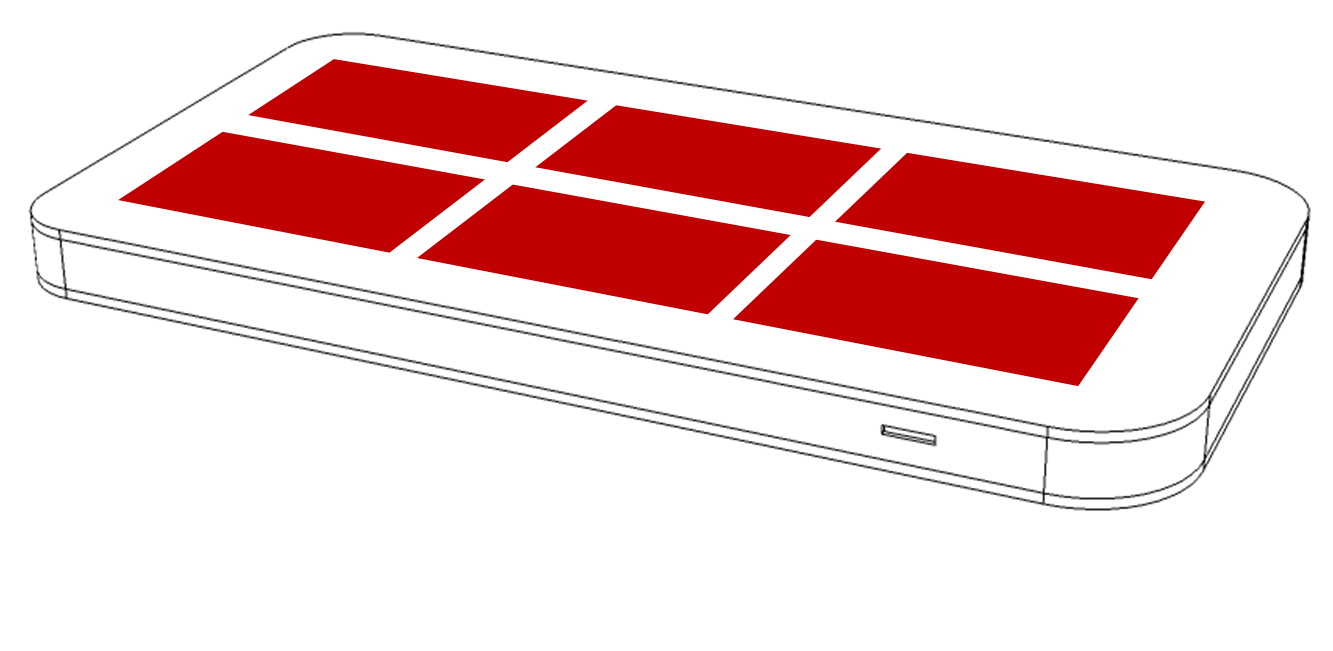
\includegraphics[width=0.6\textwidth]{images/magicbox}
\caption{MagicBox sketch - six electrodes uniformly distributed below surface}
\label{fig:magicbox_sketch}
\end{figure}
%Figure 28 MagicBox sketch - six electrodes uniformly distributed below surface
The so-called MagicBox was our first attempt to create an interaction device based on capacitive proximity sensing. It is using an array of six individual wireless capacitive sensors that communicate to a central station \cite{Braun2011MultiInputDevice}. The electrodes are using a large surface area and are made of aluminum foil. A sketch is shown in Figure \ref{fig:magicbox_sketch}. The system is able to track the position of a single hand in three dimensions up to a distance of approximately $20cm$, and uses different methods to infer gestures from the hand movement. 
It is designed to be a generic interaction device that can potentially be hidden below non-conductive surfaces. As it can be used without touching it is also applicable in sterile environments. A suite of demonstration applications has been created that showcase typical scenarios for the MagicBox. This includes multimedia applications, like image viewer and media player but also a 3D object viewer intended as demonstrator for potential medical applications, allowing a surgeon to check MRT or CT images in a sterile environment without touching any surface.

\subsubsection{Evaluation}
\begin{figure}[h]
\centering
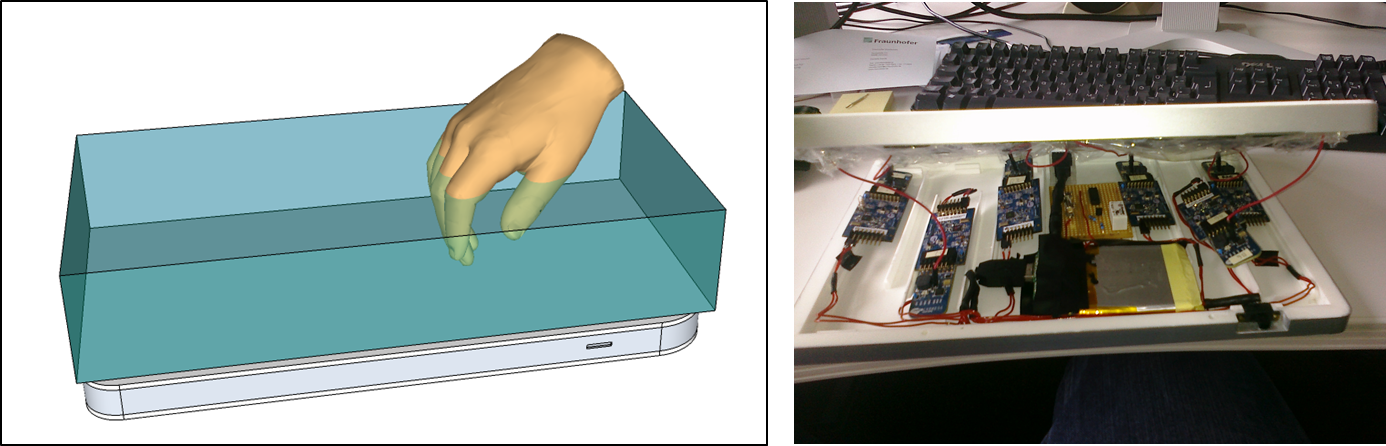
\includegraphics[width=0.8\textwidth]{images/magicbox_proto}
\caption{MagicBox conceptual rendering (left) and detail view of electronics (right) \cite{Braun2011MultiInputDevice}}
\label{fig:magicbox_proto}
\end{figure}
%Figure 31 MagicBox conceptual rendering (left) and detail view of electronics (right) [78]
The MagicBox prototype is based on the Cypress First Touch starter kit \cite{cypressfirst} and combines six capaci-tive sensors communicating wirelessly to a single base station, that are put together with a USB-rechargeable power supply into a casing. A concep-tual rendering showing the interaction area and a detail view of the prototype electronics are shown in Figure \ref{fig:magicbox_proto}.
\begin{figure}[h]
\centering
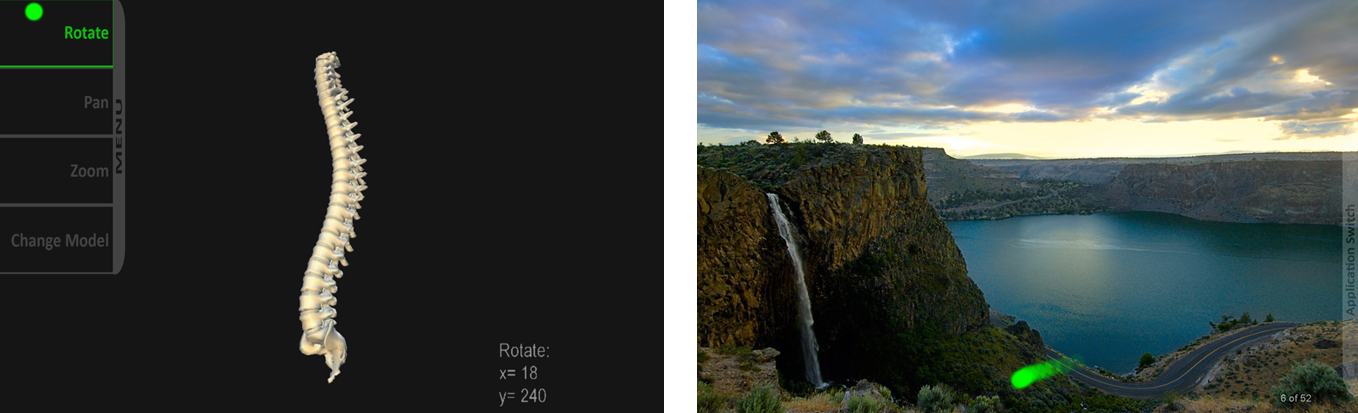
\includegraphics[width=0.8\textwidth]{images/magicbox_eval}
\caption{MagicBox demonstration application - 3D object viewer (left) and image viewer (right) \cite{Braun2011MultiInputDevice}}
\label{fig:magicbox_eval}
\end{figure}
%Figure 32 MagicBox demonstration application - 3D object viewer (left) and image viewer (right) [78]
The different iterations of the MagicBox have been evaluated in conjunction with various demon-stration applications. A usability study with 18 per-sons led to general approval of the system \cite{Braun2011MultiInputDevice}. Two of the applications used in this study are shown in Figure \ref{fig:magicbox_eval}. On the left is a 3D object viewer that has to be controlled by a combination of menu and direct manipulation of the screen content. On the right side there is an image viewer that was controlled by gesture to trigger the next/previous images or perform zooming operations. The most common positive remarks gathered in this study can be roughly put into three groups:
\begin{itemize}
\item{The device very intuitive to use}
\item{The idea of interacting this way is novel and interesting}
\item{It is easy to control applications with those gestures}
\end{itemize}
Likewise we identified three main groups for negative comments about the prototype:
\begin{itemize}
\item{The device is not very precise}
\item{The interaction speed is slow}
\item{It can be tiring for the arm}
\end{itemize}
Later iterations have been trying to improve some of the weaknesses presented above, e.g. by using a more sophisticated gesture recognition system and faster sensor refresh rates. Accordingly there were fewer complaints about interaction speed and precision \cite{braun2013capacitive}. However, the final complaint about the device being tiring for the arm, requires a different approach, that we are investigating in the final prototype to be presented in this system.

\clearpage
\subsection{CapTap}
\begin{figure}[h]
\centering
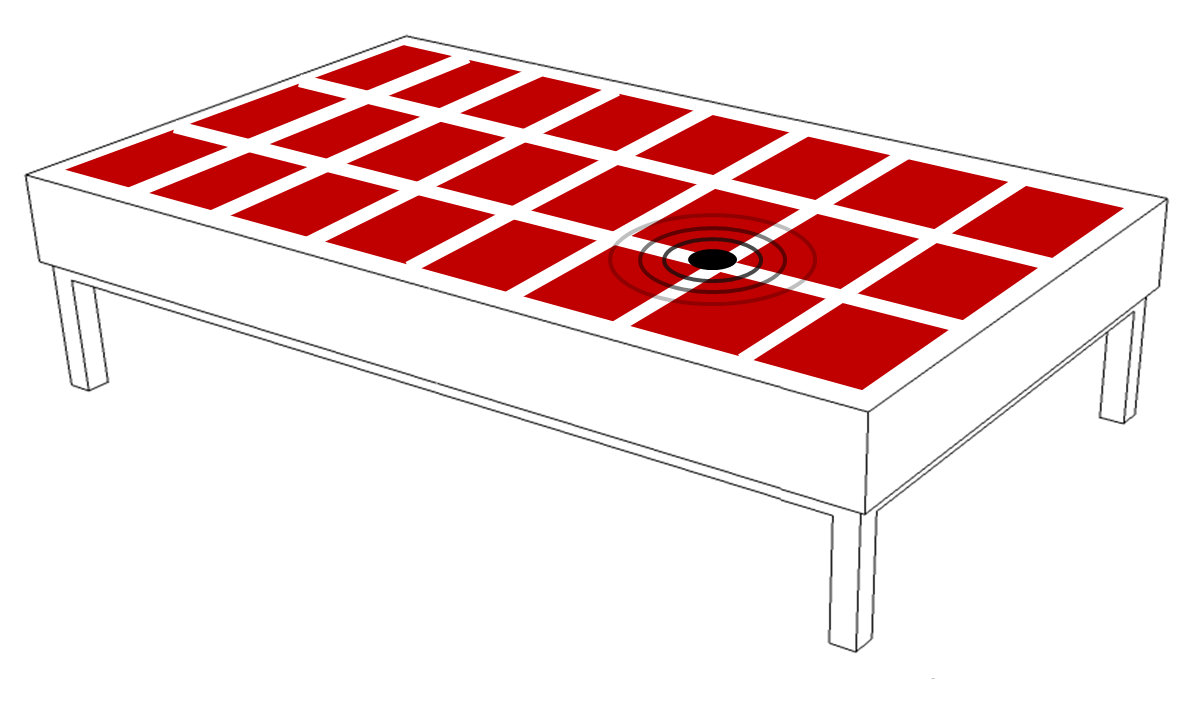
\includegraphics[width=0.7\textwidth]{images/captap_v2}
\caption{CapTap sketch - 24 electrodes placed under table surface and a single detector for touch events}
\label{fig:captap_sketch}
\end{figure}
A general insight of free-air gestural interaction that became apparent even in early works is the physical demands of prolonged interaction with such systems \cite{Baudel1993, lenman2002} and the difficulty to adapt selection events to gestural input - the latter typically being realized by time- or position-based gestures \cite{Baudel1993,Krum2002}. There is no trivial solution to this challenge and any approach has to take into account the specific application scenario covered. Some systems attempt to provide specifically adapted graphical interfaces, while others include additional input devices assisting the interaction \cite{Wu2003,zimmerman1987hand}. A major point is decreasing the required time for interaction, e.g. by adding a tactile feedback to the interaction system, preventing time-based selection gestures. CapTap is a regular living room table that includes a capacitive proximity sensor array for tracking the position of one or more arms. As it is difficult for this sensor category to detect touch, if the interaction surface is at a distance from the electrodes, a hidden acoustic system is added that allows recognizing different touch events. CapTap tracks hand and arm position using the image-based object recognition previously presented and fuses this data with different touch events generated by a single contact microphone that analyzes the audio signals in frequency space. This allows to significantly reduce interaction time, as opposed to systems relying on time-based dwell gestures. The system was created in 2013 and 2014 with collaboration of several students, most notably Sebastian Zander-Walz and Stefan Frank \cite{Braun2013captap}. It is used and further developed within the European research project POSEIDON that aims at providing technical solutions to help persons with Down's syndrome on planning their day, as input device that allows interaction regardless of motoric skill level.
\subsubsection{Capacitive layout}
\begin{minipage}{\linewidth}
\centering
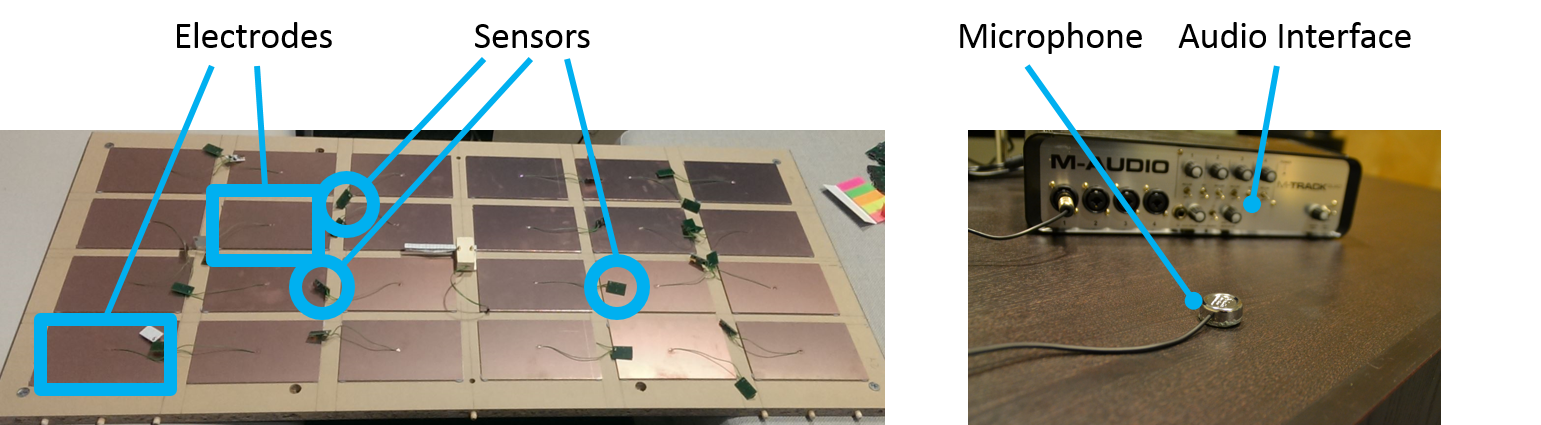
\includegraphics[width=0.8\textwidth]{images/prototype_views_new}
\captionof{figure}{Detail views of the prototype system: left - electrodes and sensors, right - audio interface and contact microphone}
\label{fig:prototype_views_new}
\end{minipage}	
 
Our goal with CapTap is to enable tracking of hands and arms that move above a table. Therefore, the electrodes are placed in an uniform array that provides similar sensing properties for the whole surface. It is realized as a prototype installed in a regular living room table. It is comprised of an array of capacitive proximity sensors, a contact microphone for touch event detection and a miniature PC. All devices can be integrated into the table in a way that it is not distinguishable from the not-augmented piece of furniture. Figure \ref{fig:prototype_views_new} shows some detail views of the disassembled prototype. The left image shows the back of the wooden tabletop. The electrodes are arranged in a 6x4 array and each one is attached to a single sensor. The right picture shows the touch detection microphone. It is attached in the center of the surface, as to avoid non-uniform sound distribution over the surface area that would be more difficult to train. Placing the microphone below the surface has no strong influence. However, a specific training phase is required for any novel surface that is equipped with the touch detection devices. 

\begin{minipage}{\linewidth}
\centering
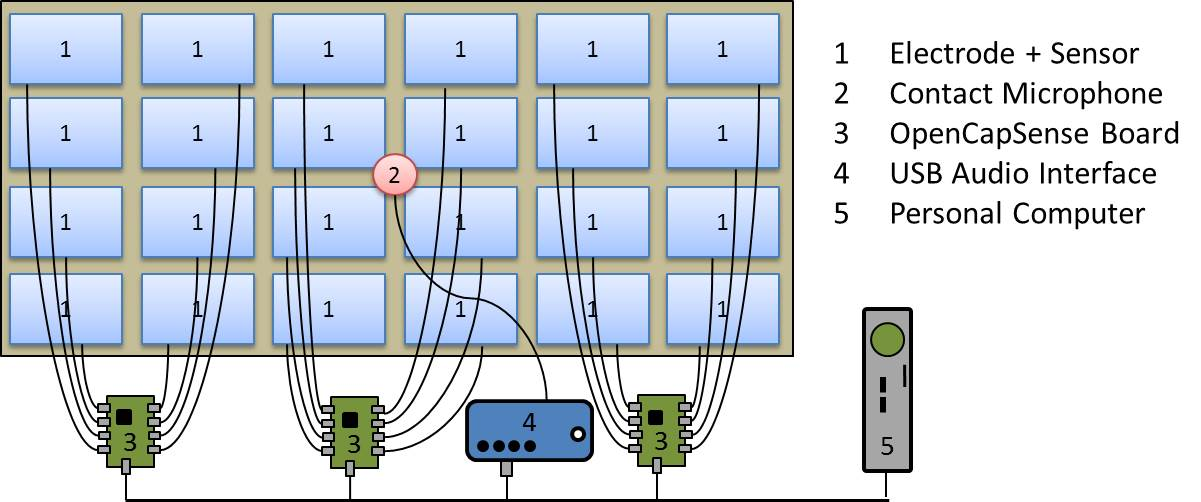
\includegraphics[width=0.8\textwidth]{images/captap_schematics}
\captionof{figure}{Abstract view below the surface of the prototype including capacitive sensing electrodes and touch detection microphone}
\label{fig:captap_schematics}
\end{minipage}

The setup is visualized in Figure \ref{fig:captap_schematics}. The system is comprised of 24 electrode \& sensor pairs that are connected to three different measurement boards. The microphone is attached to a USB Audio Interface. Overall there are four different boards connected via USB to a  PC that executes and merges the different types of data processing and links it to the software suite. The prototype is based on OpenCapSense, a more advanced prototyping system presented by Grosse-Puppendahl et al. \cite{grosse2013opencapsense}. The boards are performing some prefiltering, whereas the image-based hand tracking is realized on an attached PC. The microphone is attached to an USB audio interface (M-Audio M-Track Quad) that transfers data acquired by up to four microphones and provides various pre-sampling functions. All four devices are attached to a Mini-PC that is performing subsequent data processing and is running the demonstration and testing applications. 
 
\begin{minipage}{\linewidth}
\centering
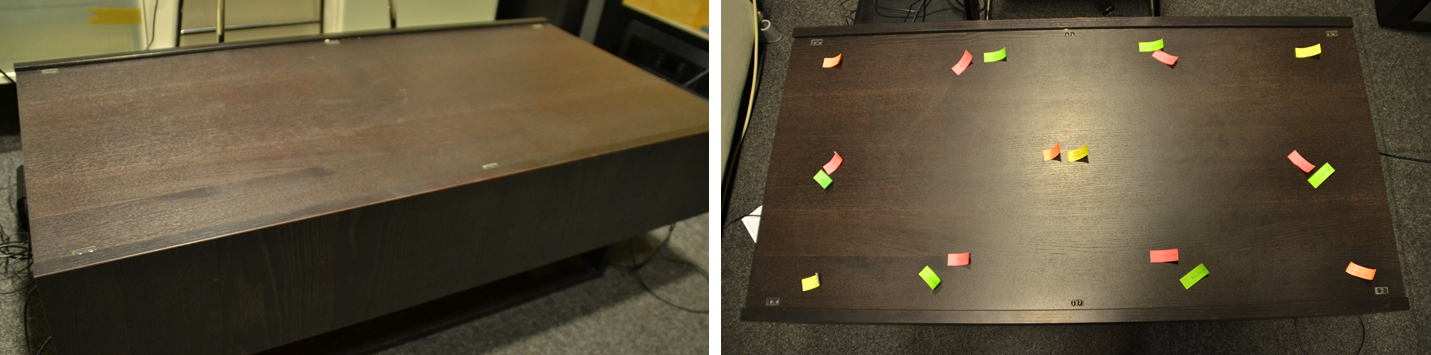
\includegraphics[width=0.8\textwidth]{images/table_final_view}
\captionof{figure}{Views of final prototype, complete view (left), top view with markers for touch evaluation (right)}
\label{fig:table_final_view}
\end{minipage}

The final table prototype can be seen in Figure \ref{fig:table_final_view}. On the left side the table is seen without any additional markers - on the right side we see the table equipped for the evaluation using a set of markers for different touch and swipe events. The debug software was developed with C\# using the .NET 4.5 framework. We are using the Emgu CV library based on OpenCV for image processing and application of the Kalman filter to the determined palm locations. The sound processing is implemented in C++ and Java using a modified version of ChucK for audio sampling and the WEKA framework to apply the machine learning on top. We are using sockets to transfer data between the different modules. The debug application allows a fine control of the various processing steps in both image and audio signal processing.

%\begin{minipage}{\linewidth}
%\centering
%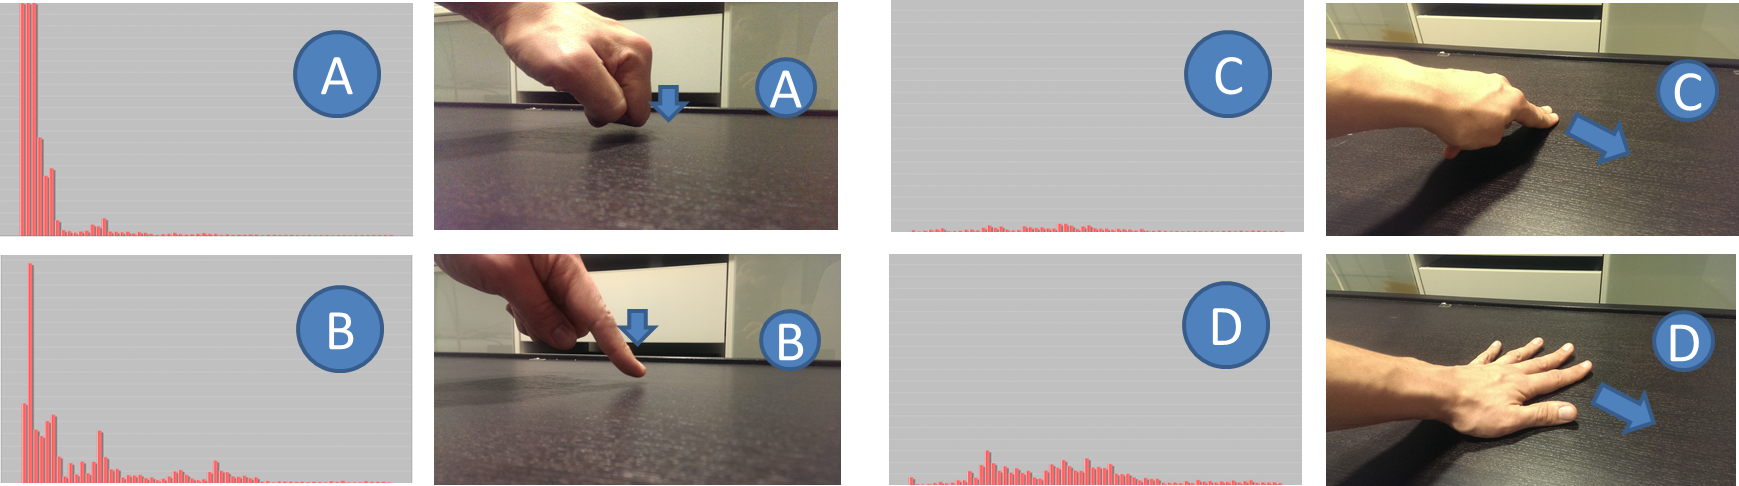
\includegraphics[width=1.0\textwidth]{images/alltouch}
%\captionof{figure}{64 sample FFTs and photo for a knock event (A), a finger tap (B), a finger swipe (C) and a hand swipe (D)}
%\label{fig:alltouch}
%\end{minipage}

\subsubsection{Processing}
CapTap is using the image-based algorithm for tracking palms and arms that was presented in the processing section. An addition is the touch recognition based on acoustic tracking. The method was inspired by the works of Harrison et al. \cite{harrison2011tapsense} with various modifications to allow identifying both impact and swipe events. At first the audio signal is acquired using a 96kHz sample rate and a feature extraction rate of 375Hz (using a  Hanning type sliding window of 4096 (and 256 samples overlapping) samples per extraction. In order to perform a classification over this signal we have to look at a variety of different features.
\subsubsection*{Feature vector}
The signal differences are most significant in the frequency domain, thus we are performing a FFT over 4096 samples, looking at the first 512 of 2048 magnitude values, thus covering the frequency range up to 12kHz. We are collecting the mean value, the standard deviation and the index of the highest value within the frequency range. This process is repeated for a downsampled FFT of 64 values, similar to the method used by Harrison et al. Another frequency domain-feature we are using is the centroid, i.e. the weighted mean of the present frequencies. Additionally, we are using two time-domain features, the RMS power (root mean square), i.e. the average magnitude within the current frequency band and the number of zero crossings of the signal. 
\subsubsection*{Classification}
We have to distinguish two different classifiers that are used for impact and swiping events. Even though knocks and taps are temporal gestures they are short in duration, while the swipe gestures are constant for a longer time period. Example 64-value FFTs are shown in Figure \ref{fig:alltouch}, with impact events and their low-frequency peaks on the left and swipe events and their fairly constant value on the right. For impact events we are using some metrics to identify the point at which the features shall be analyzed. A simple preprocessing identifies increasing power in lower frequencies and begins to store all feature vectors until a maximum is reached or the power is decreasing again. Not relevant secondary power increases (that are prevalent on stronger knocking events) are ignored. The feature vector corresponding to the maximum is then put into the classifier. This is a trained SMO classifier comprised of a support vector machine and a polynomial kernel that matches five different impacts - single knock, double knock, single finger tap, single double tap, and stomps that are classified but not used any further.
The classification of different swipe events is realized using a sliding window over a set of previous feature vectors. The derived feature set is comprised primarily of average and standard deviations of the single items within the previous feature vectors. The FFT values are most relevant. This combined feature set is fed into a decision tree that is using several thresholds to decide if the swipe was performed by a finger or the whole hand. We are using the effect that swipes have fairly constant values in the frequency band between 2kHz and 8kHz. This classification is performed each 256 samples. In order for a swipe gesture to be identified a number of subsequent positive classifications have to occur. For example 10 classifications that indicate a constant movement of 26ms or more are identified as a swipe gesture.

\subsubsection{Evaluation}
In order to evaluate our system we have performed a combined study by 10 users who were invited to test the accuracy of the touch detection and benchmark the interaction speed. They predominantly had plenty of experience with touch devices (all questionnaire questions refer to Likert-scale 1 to 10, $\mu=9.40, \sigma=1.90$). Experience with gesture interaction systems like the Kinect or Leap Motion was less prevalent and had a higher variation ($\mu=6.00, \sigma=2.71$).
 
\begin{minipage}{\linewidth}
\centering
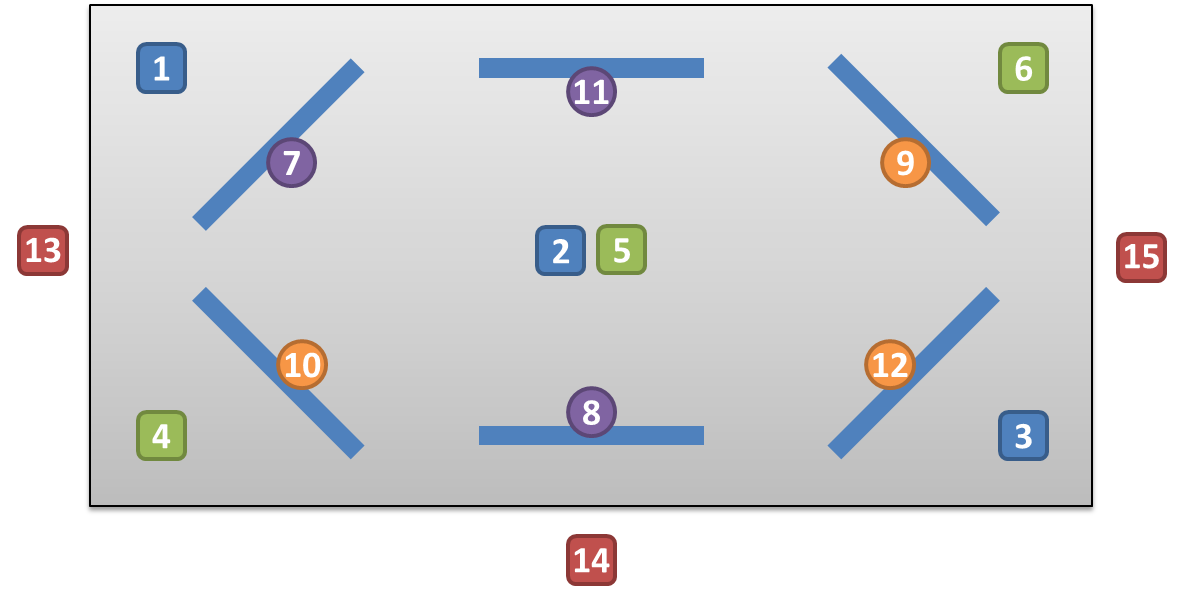
\includegraphics[width=0.8\textwidth]{images/eval_touch_v2}
\captionof{figure}{Finger tap (blue), knuckle knock (green), finger swipe (purple), hand swipe (orange) and stomping (red) spots relative to tabletop.}
\label{fig:eval_touch_v2}
\end{minipage}

\subsubsection*{Touch detection accuracy}
One of the main interesting aspects for us is the accuracy of the touch detection with a classification that is only trained by a limited number of users. Six different types of touch events are tested by the different users - finger tap, double finger tap, knuckle knock, double knuckle knock, finger swipe and hand swipe. In addition we want to get an idea if outside influences can disturb the signal, thus we are letting the users stomp at three different locations in close proximity of the table. Overall we have 12 different areas on the table that have to be touched in different ways by the users. These are executed three times each, leading to 54 touch samples and 9 stomp samples. The locations shown in Figure 12  are (double) finger taps (1,2,3), (double) knuckle knocks (4,5,6), finger swipes (7,8,9), hand swipes (10,11,12) and  stomps (13,14,15). The main purpose of this evaluation was to test a pre-trained algorithm that does not require any training efforts by the user. The subjects were shown all different supported touch gestures just once in a live example. The results are shown in Table \ref{tab:prot_captap_eval_knock}. The system was very well capable of recognizing the different taps having a success rate of 96\% or more. The results were not as good for knock detection, with only 81\% correct classification of single knocks and 60\% correct classification of double knocks. However, it should be noted that there was a high variance in results.
 
\begin{table}[htbp]
  \centering
  \caption{Results of touch detection for single and double taps (SFT, DFT), knocks (SKK, DKK), finger swipe (FS), hand swipe (HS) and stomp (STO). Noted are the overall samples, errors, no event errors, wrong classification errors and the percentage of correct classification.}
    \begin{tabular}{lccccccc}
    \toprule
          & \textbf{SFT} & \textbf{DFT} & \textbf{SKK} & \textbf{DKK} & \textbf{FS} & \textbf{HS} & \textbf{STO} \\
    \midrule
    \textbf{Samples} & 90    & 90    & 90    & 90    & 90    & 90    & 90 \\
    \textbf{Errors} & 1     & 3     & 17    & 36    & 18    & 2     & 22 \\
    \textbf{No event} & 1     & 0     & 0     & 0     & 6     & 0     & 0 \\
    \textbf{Wrong Class} & 0     & 3     & 17    & 36    & 12    & 2     & 22 \\
    \textbf{Percentage correct class} & 98,89 & 96,67 & 81,11 & 60    & 80    & 97,78 & 75,56 \\
    \bottomrule
    \end{tabular}%
  \label{tab:prot_captap_eval_knock}%
\end{table}%

Two users accounted for half the errors of double knock recognition as none of their double knocks were recognized. Thus with some additional training and adaptation it should be possible to detect all knocks. The classification of finger swipes showed similar results. The majority of errors (15 of 18) were produced by a small set of subjets (3 of 10), leading to a detection rate of only 80\%. Again, training the different gestures should lead to an improvement. The results for hand swipe were very favorable with a detection rate of almost 98\%. Stomps were able to disturb the system in about 25\% of all events. However, in practical applications they are not highly relevant, as we can rule out any events where no hand is present above the table. Our tests showed that it is also very important to consider the uniformity of the table. The recognition rate of finger swipes at position 8 (93.33\%) was considerable better than the recognition at positions 7 and 9 (73.33\% for both), indicating that it is important to test each touch gesture at various positions and adjust the algorithm accordingly.
\subsubsection*{Hand tracking and interaction speed}

\begin{minipage}{\linewidth}
\centering
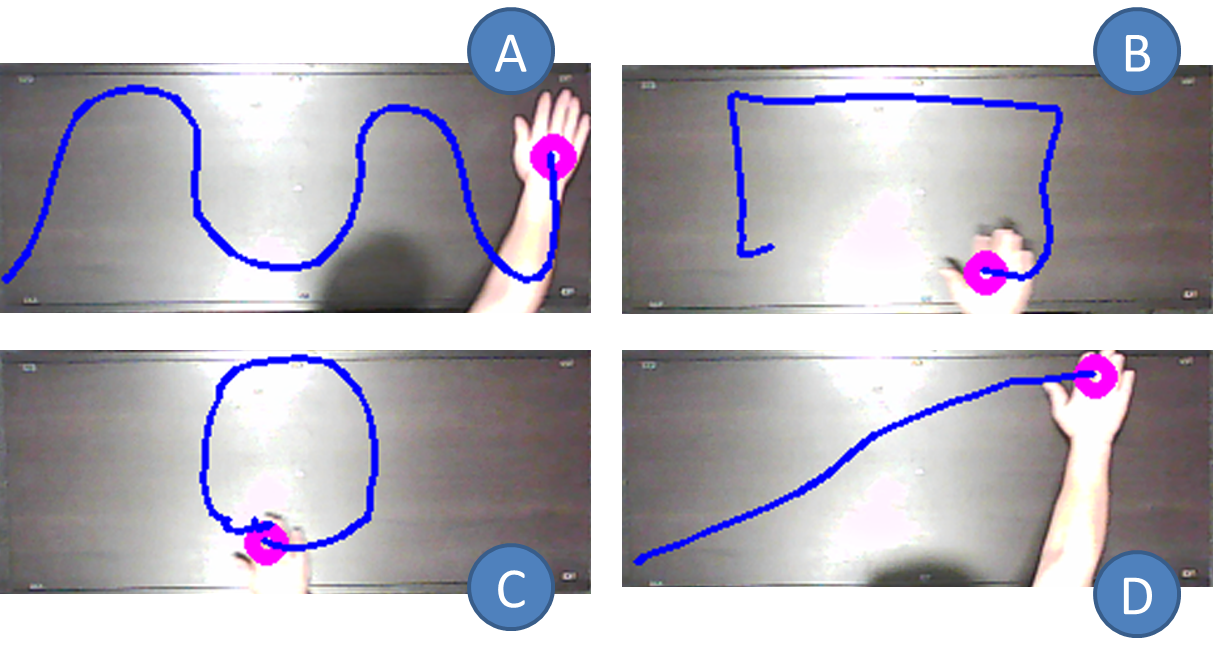
\includegraphics[width=0.8\textwidth]{images/tracks}
\captionof{figure}{Tracks generated by Kalman filtered palm position, a sine wave (A), a rectangle (B), a circle (C), and a diagonal swipe (D)}
\label{fig:tracks}
\end{minipage}

In order to properly identify gestures the recognized paths of the hands are the most important measure. We have added a visualization module to the registered camera image introduced previously that allows us to show the tracks followed by one or more hands. Figure \ref{fig:tracks} shows several of the paths that were generated this way using single hand tracking. The hand is in this case moving about 10-15 cm above the table surface. While we have not connected the system to a generic path-based gesture recognition system, we can see that the system can create smooth trajectories that can be analyzed further.

A major point of interest for us was to check if users could successfully use the layer interaction pattern introduced before and if the option for adding unobtrusive touch detection would have any influence on the interaction speed. For this we used a small game whereas the participants had to put a cursor into a box and perform either a dwell (approximately 300ms) or touch activity for selection. The cursor reflected the current interaction layer by color coding. We counted the time it took to complete a run of 15 boxes.

\begin{minipage}{\linewidth}
\centering
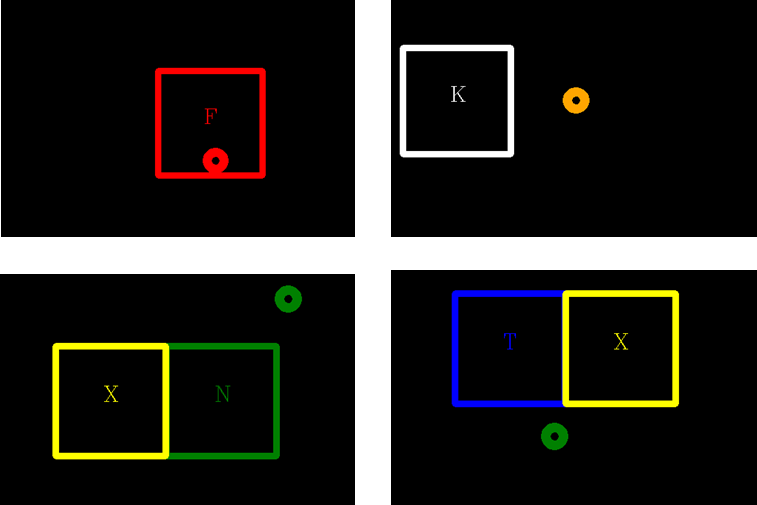
\includegraphics[width=0.8\textwidth]{images/eval_speed}
\captionof{figure}{Interaction speed evaluation. Different types of boxes for near layer (N), knock (K), far layer (F), and disturber (X).}
\label{fig:eval_speed}
\end{minipage}

Some example boxes are shown in Figure \ref{fig:eval_speed}. There were six different types referring to dwelling in the three different layers, knock, tap and disturber. Each participant performed four runs. First a training run, then a run with all interaction layers and the two touch events, then a run with dwelling boxes only (without layers), and finally a run with tap boxes only. The dwell and tap runs also included some disturber boxes to slightly increase the challenge. The order of the runs were switched equally between the different participants. Regarding the full interaction run we wanted to know if the user understands the different layers and can achieve a good interaction speed. The main hypothesis we wanted to test was that tapping improves the interaction speed as opposed to dwelling and may reduce the overall interaction times, thus reducing potential fatigue. We expected the tap run to be shorter than the dwell run as selection events can be performed faster. All runs had the same overall distance and the last two had inverse order to account for Fitts’ law.

\begin{table}[htbp]
  \centering
  \caption{Results for interaction time in the different runs of the interaction speed test}
    \begin{tabular}{lccc}
    \toprule
          & \textbf{Full run} & \textbf{Dwell run} & \textbf{Tap run} \\
    \midrule
    \textbf{Average Time} & 40.12 & 37.97 & 33.42 \\
    \textbf{Shortest Run} & 27.28 & 32.20 & 24.29 \\
    \textbf{Longest Run} & 51.38 & 48.11 & 47.72 \\
    \textbf{Standard Deviation} & 7.22 & 5.27 & 7.93 \\
    \bottomrule
    \end{tabular}%
  \label{tab:prot_captap_eval_intspeed}%
\end{table}%

The results are shown in Table \ref{tab:prot_captap_eval_intspeed}. Running a paired t-test on dwell and tap run the resulting p value is 0.0071, indicating a high statistical significance that the interaction using taps is faster than the interaction using dwelling. This fits expectations from literature [24]. While this can be countered by reducing the dwell time, the risk of wrongful selection of nearby objects increases significantly.
Questionnaire
Finally, we asked all participants to fill in a questionnaire with Likert questions in the style mentioned at the beginning of this section. Most users considered the device to be easy and precise enough to use ($\mu=8.1, \sigma=1.52$) and considered it highly intuitive ($\mu=8.9, \sigma=0.74$). Regarding the layer model they had no problem using it in the full test run ($\mu=8.6, \sigma=0.97$) but were critical to adding more layers ($\mu=3.9, \sigma=2.08$). They clearly preferred ($\mu=2.6, \sigma=2.72$) finger taps (Likert score 1) to knocks (Likert score 10). There was no clear preference for finger swipes (score 1) or hand swipes (score 10) ($\mu=4.6, \sigma=3.06$). The participants considered CapTap to be an interesting interaction device ($\mu=9.1, \sigma=1.20$) and could even imagine using it for longer periods ($\mu=6.9, \sigma=1.97$). Asking for particular points that they liked about the current version of CapTap the comments mentioned the ease of use and the high variety of different input commands that are supported. Points that were disliked are the usage of knocks that were considered unpleasant after a short while, even during the 10 minute study that only included few knocks. The hand tracking at this point is sometimes disturbed by the user’s knees that enter the generated electric field around the table.



\clearpage
\section{Other capacitive prototypes}
\label{ch:prot_otherprot}
In collaboration with other partners from industry and different students some additional prototypes have been created that are discussed briefly in this section. 

\begin{figure}[ht]
\centering
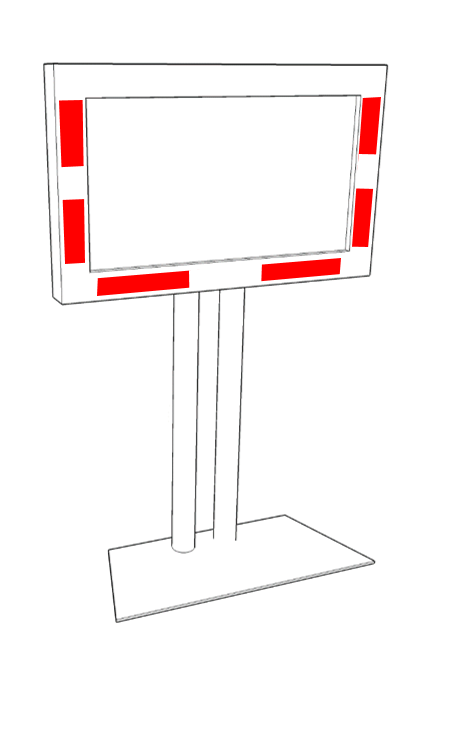
\includegraphics[width=0.4\textwidth]{images/other_proto_capdisp}
\caption{CapDisp sketch - TV on a stand equipped with capacitive sensors hidden below a plastic cover}
\label{fig:other_proto_capdisp}
\end{figure}

CapDisp is a presentation display augmented with capacitive sensors to enable touch-free control of several applications. It was created as a prototype for Hessen IT GmbH in 2010. The system is comprised of six Cypress CY3271 capacitive sensors that are powered via USB and interfaced to a Mini-PC that is attached behind a 42" display on a presentation stand, as shown in a sketch in Figure \ref{fig:other_proto_capdisp}. The display is set in an additional case that hides the six electrodes that are made of copper foil. As shown in Figure \ref{fig:other_proto_capdisp}, they are placed on the bottom and right part of the screen, allowing to detect four different swiping gestures, left and right on the bottom of the screen, up and down on the left side of the screen. The gestures can be performed at a distance of up to 20cm in front of the electrodes. Since the primary purpose of this device is showing presentations, some additional dwell gestures were added, that allow jumping to the first or to the last slide by holding the hand in front of a specific sensor for a certain time. Additionally, two other applications were included, a gesture-controlled image viewer and a video player.

\begin{figure}[ht]
\centering
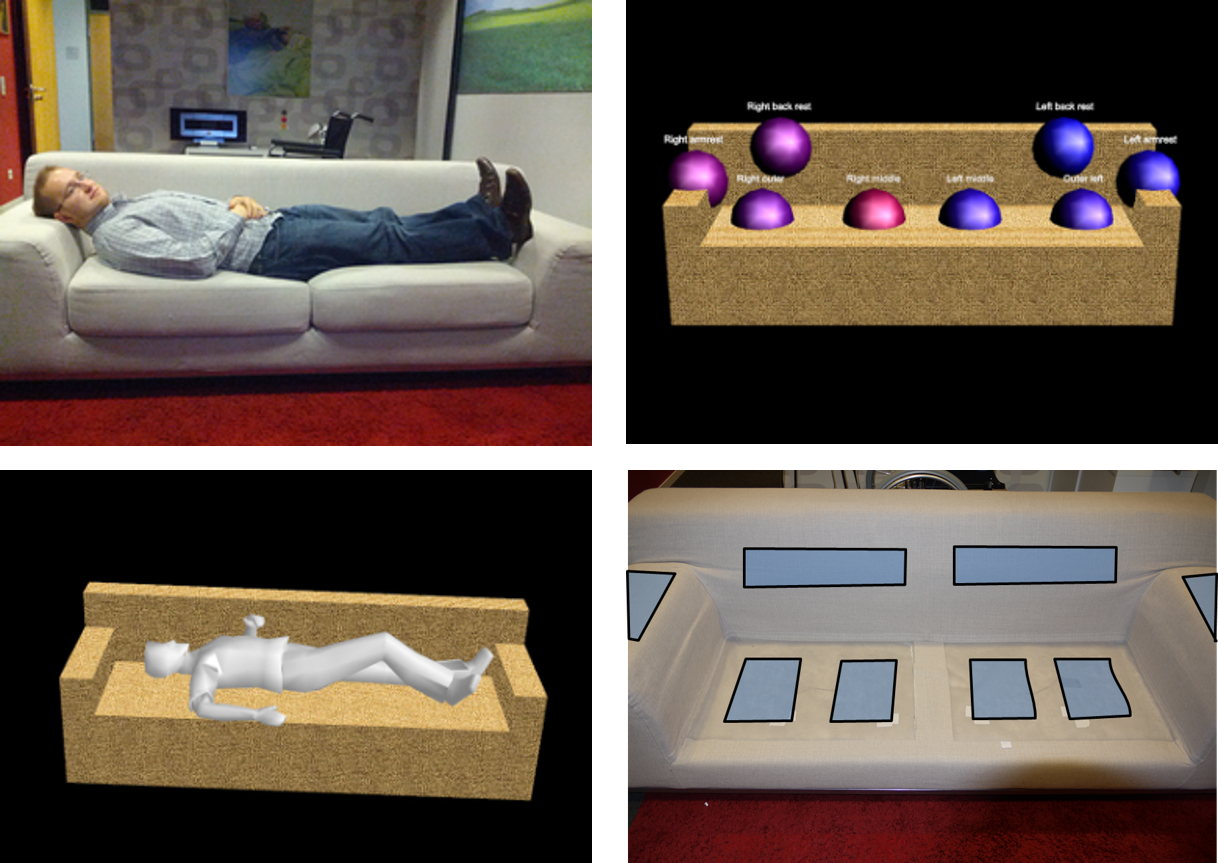
\includegraphics[width=0.8\textwidth]{images/other_proto_smartcouch}
\caption{\emph{Top left}Person lying on the couch. \emph{Top right}Resulting sensor value visualization. \emph{Bottom left}Rendering of recongized posture. \emph{Bottom right}Position of electrodes within the couch.}
\label{fig:other_proto_smartcouch}
\end{figure}

The smart couch was created by then-student Tobias Grosse-Puppendahl in scope of a practical course in 2010/11, supervised by Alexander Marinc and me. The results were later published at the AmI 2011 conference \cite{Couch2011}. Using an array of eight capacitive proximity sensors that are unobtrusively placed inside a couch it is possible to determine the posture of one or more persons that are currently occupying the system. The sensor readings are calibrated and normalized and fed into the WEKA machine learning framework for classification. Three different classifiers have been tested, decision trees, Na\"{i}ve Bayes and RBF networks, whereas the latter provided the best results. The system was evaluated with 18 users and 8 resulting postures (6 with one person, 2 with two persons), such as sitting left or right, or lying in a specific direction. The resulting measurements was distinguished in a training set from 9 persons and a test set from 9 persons. The resulting precision was 97.5\%, the recall 97.2\%. The system is still working as a demonstrator in our living lab, implicitly controlling different networked systems based on the detected postures, e.g. activating ambient lighting as soon as the person is lying down.

\begin{figure}[ht]
\centering
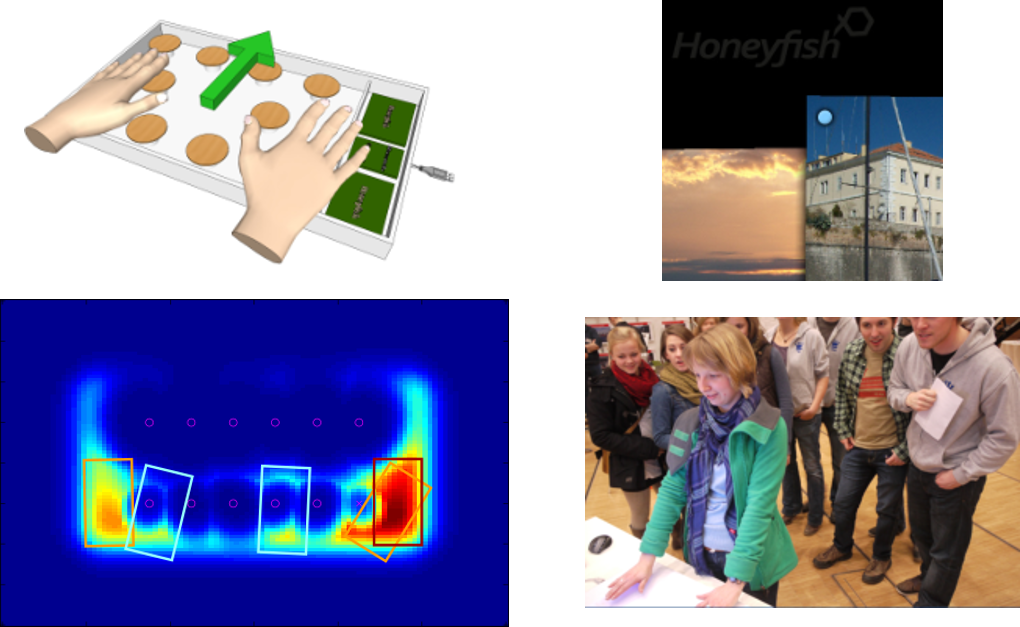
\includegraphics[width=0.8\textwidth]{images/other_proto_honeyfish}
\caption{\emph{Top left} Rendering of Honeyfish device and hands. \emph{Top right} Image of developed GUI and pointer. \emph{Bottom left} Swiss cheese algorithm predicting objects in interaction space. \emph{Bottom right} Evaluation of Honeyfish at a student fair.}
\label{fig:other_proto_honeyfish}
\end{figure}

Honeyfish is a gesture interaction device based on capacitive proximity sensors operated in shunt mode. It was created by Tobias Grosse-Puppendahl in scope of his Master's thesis that I supervised in 2012. It led to two different publications focusing on the provided contributions in multiplexing and object detection \cite{grosse2012honey}\cite{grosse2013swiss}. The system is using eight different transmitters and two receivers, leading to a set of 16 virtual sensors that are set in the middle of each receiver-transmitter combination. As shown in Figure \ref{fig:other_proto_honeyfish} on the top left, the receivers are in the center and the transmitters are placed on the outside. Using a frequency division multiplex it is possible to generate 50 samples from each virtual sensor. The system is using a method of object tracking that extends on a proposal by Smith, dubbed Swiss-cheese, which is based on the premise that each sensor not recognizing an object or a distant object is cutting a (ellipsoid) hole in the object presence probability space, thus leading to a probability distribution visually resembling a Swiss cheese \cite{Smith1996a}. The remaining probability space can be analyzed to fit hand shaped objects, thus enabling gesture detection. A particle filter is used to track the position of the hands. The system is able to track multiple hands and was used to control applications ranging from an image viewer, the GNU TuxRacer game to a remote-controlled vehicle.
\begin{figure}[ht]
\centering
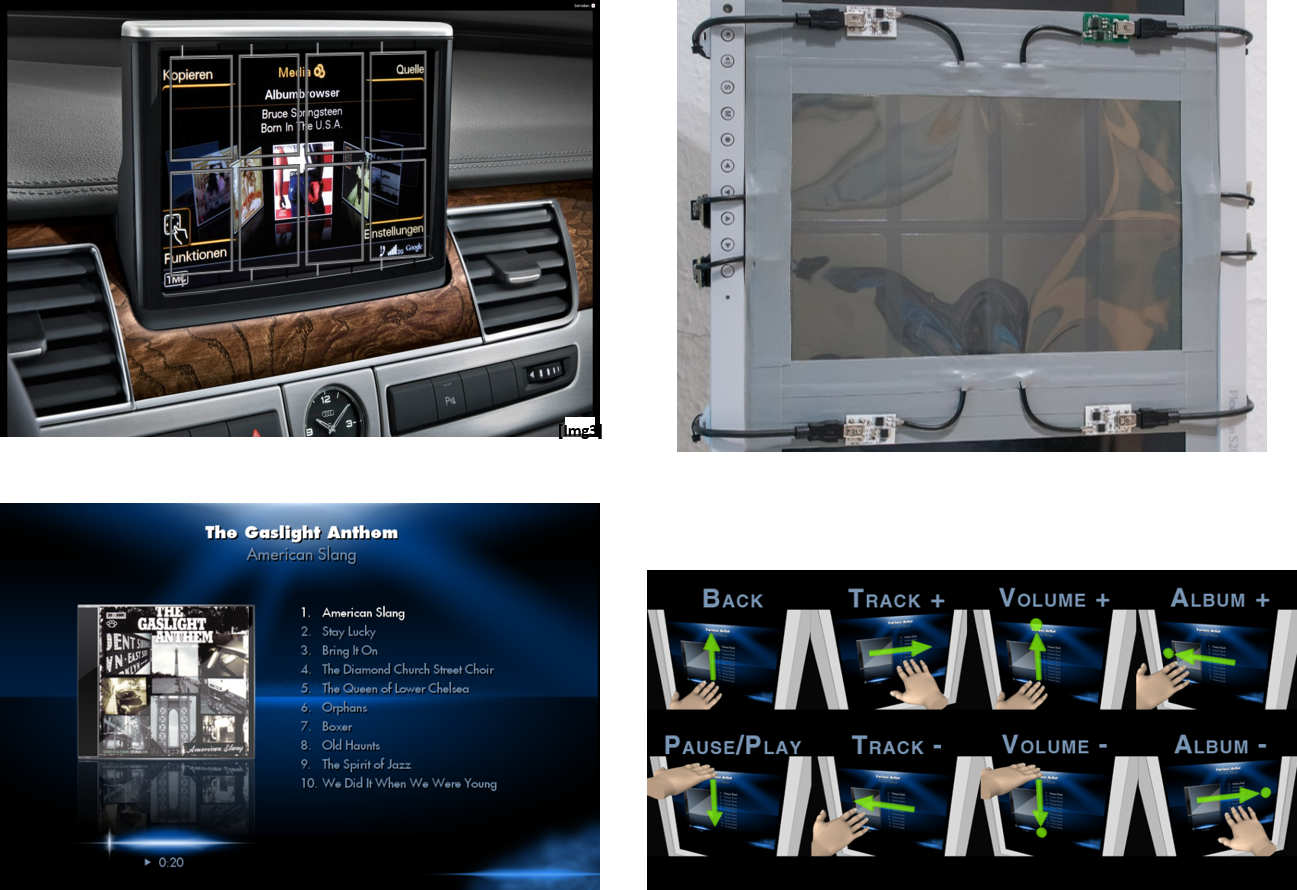
\includegraphics[width=0.8\textwidth]{images/other_proto_gestdisp}
\caption{\emph{Top left} Concept image of GestDisp in a car with outlined electrodes. \emph{Top right} GestDisp prototype installed in front of a monitor. \emph{Bottom left} Screenshot of demonstration application music player. \emph{Bottom right} Association of gestures to functions in the demonstration application.}
\label{fig:other_proto_gestdisp}
\end{figure}

GestDisp is the final prototype discussed in this work. It was created by Yannick Berghöfer in 2013 as part of his Master's thesis that was supervised by me and Tobias Grosse-Puppendahl. The basic idea is to enable gestures performed in front of a screen by applying capacitive proximity sensors on the screen surface. Consequently a different type of electrode material has to be used, that combines conductivity and transparency. Different materials have been evaluated, including ITO (indium-tin oxide) and PEDOT:PSS (a conductive polymer) in order to find a suitable electrode candidate. ITO was chosen and attached to the screen including shielding electrodes, reducing the effect of the electric components used to create this display. Nonetheless, the complex and highly disturbing environment drastically limits the distance in which gestures may be performed. The gestures are recognized using a Hidden-Markov-Model classifier that was trained by the developers.  Using this, it was possible to distinguish swipe gestures in four directions, selection gestures as indicated by dwelling at a certain position and combined swipe-and-hold gestures, whereas the hand is resting in the interaction area after performing a swipe, e.g. used for continuous scrolling or increasing the volume. The gesture recognition includes a specific garbage-gesture that allows to distinguish arbitrary movements in the interaction area from deliberate gestures and has to be trained separately. This approach allows a precision and recall of about 95\% on a collected training set. A demonstration application was created that mimics a multimedia system in a car, allowing to control different radio stations or select music of choice.  
